% chktex-file 1
% chktex-file 2
% chktex-file 3
% chktex-file 4    
% chktex-file 5
% chktex-file 6
% chktex-file 7
% chktex-file 8
% chktex-file 9
% chktex-file 10
% chktex-file 11
% chktex-file 12
% chktex-file 13
% chktex-file 14
% chktex-file 15
% chktex-file 16
% chktex-file 17
% chktex-file 18
% chktex-file 19
% chktex-file 20
% chktex-file 21
% chktex-file 22
% chktex-file 23
% chktex-file 24
% chktex-file 25
% chktex-file 26
% chktex-file 27
% chktex-file 28
% chktex-file 29
% chktex-file 30
% chktex-file 31
% chktex-file 32
% chktex-file 33
% chktex-file 34
% chktex-file 35
% chktex-file 36
% chktex-file 37
% chktex-file 38
% chktex-file 39
% chktex-file 40
% chktex-file 41
% chktex-file 42
% chktex-file 43
% chktex-file 44

\documentclass[11pt,a4paper]{article}
% Preamble moved from main.tex

\usepackage{tocloft}
\usepackage{silence}
\WarningFilter{tocloft}{\@starttoc has already been redefined}

% --- 1. Page Layout (Guidelines 4.2) ---
\usepackage[left=2cm,right=4cm,top=2cm,bottom=2cm]{geometry}
% --- FIX: Page Number Centering ---
\usepackage{fancyhdr}
\pagestyle{fancy}
\fancyhf{} % Clear default header/footer
\renewcommand{\headrulewidth}{0pt} % Remove the header line

% Calculate the offset: (Right Margin - Left Margin) / 2
% (4cm - 2cm) / 2 = 1cm
% We shift the page number 1cm to the Right to hit the true center.
\fancyfoot[C]{\hspace{1cm}\thepage}

% --- 2. Spacing and Paragraphs ---
\usepackage{setspace}
\setstretch{1.5}
\usepackage[parfill]{parskip}
\setlength{\parskip}{6pt}
\setlength{\parindent}{0pt}

% --- 3. Typography & Fonts ---
\usepackage{noto}
\usepackage{courier}
\usepackage[T1]{fontenc}
\usepackage[utf8]{inputenc}
\usepackage{microtype}
\setlength{\emergencystretch}{2em}
\hbadness=2000
\usepackage[english]{babel}
\usepackage{csquotes}
\usepackage{xcolor}
\usepackage{amssymb}
\usepackage{listings}
\usepackage[hidelinks]{hyperref}
\urlstyle{same}

% --- 4. Table of Contents Formatting ---
\renewcommand{\cfttoctitlefont}{\normalfont\fontsize{14}{17}\bfseries}
\renewcommand{\cftaftertoctitle}{}
\renewcommand{\cftsecleader}{\cftdotfill{\cftdotsep}}
\renewcommand{\cftdotsep}{1}
\setlength{\cftbeforesecskip}{6pt}

% --- 5. Headings (Guidelines 4.2) ---
\usepackage{titlesec}
\titleformat{\section}{\normalfont\fontsize{14}{17}\bfseries}{\thesection}{1em}{}
\titleformat{\subsection}{\normalfont\normalsize\bfseries}{\thesubsection}{1em}{}
\titleformat{\subsubsection}{\normalfont\normalsize\bfseries}{\thesubsubsection}{1em}{}

% --- 6. Tables and Graphics ---
\usepackage{tabularx}
\usepackage{multirow}
\usepackage{graphicx}
\usepackage{booktabs}
\usepackage{caption}
\usepackage{float}
\captionsetup{font={small}}

% --- 7. Linguistics Packages ---
\usepackage{expex}
\usepackage[nohyperlinks]{acronym}
\usepackage{blindtext}

% --- 8. Blockquotes ---
\usepackage{etoolbox}
\AtBeginEnvironment{quote}{\small\singlespacing}
\AtBeginEnvironment{quotation}{\small\singlespacing}

% --- 8.5. Code Listings (Appendix) ---
\lstset{%
  basicstyle=\ttfamily\footnotesize,
  breaklines=true,
  breakatwhitespace=false,
  columns=fullflexible,
  keepspaces=true,
  showstringspaces=false,
  frame=single,
  framerule=0.2pt,
  rulecolor=\color{black!30}
}

% --- 9. Bibliography Setup (Guidelines 5) ---
\usepackage[
    backend=biber,
    style=authoryear-comp,
    sortlocale=en,
    maxcitenames=2,
    maxbibnames=99,
    dashed=false,
    uniquelist=false
]{biblatex}

\DeclareNameAlias{sortname}{family-given/given-family}
\DeclareNameAlias{author}{family-given/given-family}
\renewcommand{\postnotedelim}{\addcolon\addspace}
\DeclareFieldFormat{postnote}{#1}
\DeclareFieldFormat[book]{series}{\mkbibparens{#1}}
\renewbibmacro{in:}{\ifentrytype{article}{}{\printtext{\bibstring{in}\intitlepunct}}}
\setlength{\bibitemsep}{6pt}
\setlength{\bibhang}{0pt}
\renewcommand*{\bibfont}{\singlespacing}
\addbibresource{bibliography.bib}

\begin{document}
\hypersetup{pageanchor=false}
\pagenumbering{roman}
\renewcommand\contentsname{Table of Contents}

% --- Title Page ---
\newgeometry{left=3cm,right=3cm,top=2cm,bottom=2cm}

\begin{titlepage}
    \centering

    
\includegraphics[width=.3\textwidth]{Images/logo_uni.png}\\[1em]
    Fakultät für Sprach-, Literatur- und Kulturwissenschaften\\[1em]
    {\Large Bachelorarbeit}\\[1em]
    {Im Studiengang Englische Sprachwissenschaft}\\[1em]
    {Sommersemester 2026}

    \vspace{5cm}

    \textbf{\fontsize{16}{19}\selectfont Can AI Replace Traditional Textbooks?}\\[0.5em]
    \large \textbf{A Comparative Corpus Analysis of LLM-Generated vs. Textbook Example Sentences}

    \vspace*{\fill}

    \begin{flushleft}
        \begin{tabular}{ll}
            \textbf{Autor:} & Simon John \\
            \textbf{Matrikelnummer:} & 2175939 \\
            \textbf{Adresse:} & Wildbachweg 5, 93059 Regensburg \\
            \textbf{E-Mail:} & simon.john@stud.uni-regensburg.de \\
            \textbf{Studiengang:} & BA Englische Sprachwissenschaft \\
            \textbf{Abgabedatum:} & \today \\
            \textbf{Gutachter:} & Dr.\ Thorsten Brato \\
        \end{tabular}
    \end{flushleft}
\end{titlepage}

\restoregeometry

% --- Front Matter ---
\newpage

% --- Abstract ---
\begin{abstract}

\noindent Can Large Language Models (LLMs) generate pedagogical input that is both register-appropriate and systematically different from traditional textbook materials? This is the question this study seeks to answer. The Natural Reference Corpus (NRC, $N = 5,483$) compiled from B1/B2 English as a foreign language (EFL) textbooks was contrasted with the Synthetic Control Corpus (SCC, $N = 1,237$), which was artificially generated by Google Gemini 2.5 Flash under the following register conditions: HIGH (formal workplace setting), NEUTRAL (instructional setting) and LOW (casual, conversational setting). For this study, the two corpora were filtered specifically for sentences containing ten selected high-frequency, highly polysemous verbs such as \textit{run, take} and \textit{make}. The verbs in these sentences were then classified as either LITERAL or IDIOMATIC via an LLM-as-a-judge protocol, which was subsequently validated through inter-rater reliability (IRR) testing ($\kappa = 0.62$). Statistical analysis confirmed three hypotheses. First, sentences generated by Artificial Intelligence (AI) yielded significantly more IDIOMATIC contexts than the textbook sentences ($\chi^2 = 143.90$, $p < 0.001$). Second, the NRC aligned most closely with the NEUTRAL subsection of the SCC ($V = 0.024$), hinting at a high use of a distinct instructional register in English textbooks. Third, rather than behaving uniformly, idiomaticity was lemma-selective in both corpora. The findings suggest that, if prompted explicitly, LLMs can approximate or even exceed textbook register behaviour. This ``naturalness'', however, depends heavily on communicative framing, rather than on model capability alone. Implications for future textbook design and AI-assisted pedagogy are discussed.

\end{abstract}
\newpage

% --- Table of Contents ---
\tableofcontents
\newpage

% --- List of Tables ---
\listoftables
\vspace{3em}

% --- List of Figures ---
\listoffigures
\newpage

% --- List of Abbreviations ---
\section*{List of Abbreviations}\label{sec:abbreviations}

\begin{center}
\renewcommand{\arraystretch}{1.15}
\begin{tabular}{@{}ll@{}}
\toprule
\textbf{Abbreviation} & \textbf{Meaning} \\
\midrule
AI & Artificial Intelligence \\
API & Application Programming Interface \\
CA & Communicative Approach \\
CEFR & Common European Framework of Reference for Languages \\
CLT & Cognitive Load Theory \\
CSV & Comma Separated Values \\
EFL & English as a Foreign Language \\
ETL & Extract, Transform, Load \\
GTM & Grammar-Translation Method \\
HIGH & High Register Condition \\
IDIOMATIC & Idiomatic Usage Label \\
IRR & Inter-Rater Reliability \\
JSON & JavaScript Object Notation \\
KWIC & Key Words in Context \\
LLM & Large Language Model \\
LITERAL & Literal Usage Label \\
LOW & Low Register Condition \\
MDA & Multi-Dimensional Analysis \\
NEUTRAL & Neutral Register Condition \\
NLP & Natural Language Processing \\
NLTK & Natural Language Toolkit \\
NONE & Invalid Context \\
NTP & Next-Token Prediction \\
NRC & Natural Reference Corpus \\
POS & Part-of-Speech \\
PPO & Proximal Policy Optimization \\
RLHF & Reinforcement Learning with Human Feedback \\
SCC & Synthetic Control Corpus \\
\bottomrule
\end{tabular}
\end{center}

\newpage
\section*{List of Abbreviations}

\begin{center}
\renewcommand{\arraystretch}{1.15}
\begin{tabular}{@{}ll@{}}
\toprule
\textbf{Abbreviation} & \textbf{Meaning} \\
\midrule
\phantom{IDIOMATIC} & \phantom{Common European Framework of Reference for Languages} \\[-\normalbaselineskip]
TEC & Textbook English Corpus \\
QA & Quality Assurance \\
XML & eXtensible Markup Language \\
\bottomrule
\end{tabular}
\end{center}

\newpage

\hypersetup{pageanchor=true}
\pagenumbering{arabic}

% --- Main Content ---
\section{Introduction}\label{sec:introduction}

\subsection{Background \& Motivation}

Recently, the integration of Large Language Models (LLMs) into the language learning classroom is heavily reshaping how pedagogical content can be produced and distributed. In practical terms, this means that language learners are no longer limited to studying with example texts in textbooks, but can request context-specific alternatives on demand. While this development creates new opportunities for adaptive learning, it also reopens the discussion about a persistent question in applied linguistics: how closely do pedagogical examples resemble authentic language use in everyday communication?

This question is significant because traditional ``Textbook English'' has long been criticised for being overly stiff and unnatural \parencite{conti2016ugly}. Traditional learning materials tend to be explicit in meaning and syntactically strict, presenting a ``saniti(s)ed'' \parencite[13]{curdt-christiansenLanguageIdeologyEducation2015} version of English that rarely matches how speakers actually interact with each other. Here, Generative Artificial Intelligence (AI) offers a promising solution by generating ``natural, casual'' English when prompted accordingly. The question is, however, whether LLMs can truly recreate the phraseological nuances of authentic speech, or if they simply produce a statistically average imitation that is just as artificial and ``sanitised'' as the textbooks they aim to replace.

This tension between teachability and authenticity is not only about style. If learning materials overwhelmingly contain explicit grammatical and syntactical transparency over natural phraseology, learners receive input that is clear, but does not represent how language in different social contexts works. This is bound to cause intelligibility issues in real-world situations outside the English as a foreign language (EFL) classroom. Register-oriented \parencite{biber1988variation, leFoll2021b} and phraseological research \parencite{sinclairCorpusConcordanceCollocation1991} therefore provide an appropriate basis for an empirical study on this issue.

\subsection{Research Gap \& Study Rationale}

Most recent work regarding AI in education focuses on the technology as an evaluator, assistant or interactional partner for learner output \parencite{holmesArtificialIntelligenceEducation2019}. In contrast, comparatively little research has been conducted on AI as a robust provider of pedagogical input. This is the central gap this thesis addresses.

The secondary gap is methodological. Claims that AI output either sounds ``natural'' or ``unnatural'' are often made intuitively without actual testing through objective corpus linguistics procedures. To move on from subjective intuition to quantitative evidence, this thesis operationalises authenticity through measurable linguistic dimensions, specifically focusing on register distribution \parencite{biber1988variation} and patterns in idiomaticity \parencite{sinclairCorpusConcordanceCollocation1991}.

From the perspective of language acquisition, the relevance of this gap is very practical. The input quality has a direct impact on what learners can notice and acquire over time \parencite{krashenInputHypothesisIssues1985}. Even though this study does not measure cognitive load directly, it acknowledges that wording, phraseology and information packaging play a fundamental role in cognitive processing in educational contexts \parencite{spiroCognitiveFlexibility1992, swellerCognitiveLoadProblem1988a}.

\subsection{Research Question \& Design Overview}

This study uses a data-driven approach, utilizing methods of Corpus Linguistics to address the following research question: \textit{To what extent can Large Language Models (specifically Gemini 2.5 Flash) generate linguistically distinct registers (formal, instructional and casual) that quantitatively differ from human-authored textbook materials?} To answer this question, this study takes an existing Natural Reference Corpus (NRC), compiled by Le Foll \parencite*{leFoll2021a} from EFL textbook materials and compares it to a Synthetic Control Corpus (SCC). The SCC is generated by Google's Gemini 2.5 Flash Application Programming Interface (API) via role-prompting across three distinct registers: formal workplace language (HIGH register: questions and professional contexts), instructional language (NEUTRAL register: imperatives, directives and rules) and casual conversational language (LOW register: statements in informal contexts). The comparative nature of this study enables testing for alignment between textbook English and the AI generated formal, instructional or casual registers. It might also reveal, if textbooks have a distinct pedagogical register unlike any of these.

In analytical terms, the comparison between the two corpora is made on sentence level, focusing on ten high-frequency, polysemous verbs (e.g., \textit{run, take, make}). As such verbs are both common and semantically flexible \parencite[54--55]{stoeckelNGSL2019}, research of their occurrences in literal versus idiomatic contexts will provide a quantifiable metric for phraseological authenticity. By tracking how these verbs shift between transparent, literal meanings and de-lexicalised, idiomatic chunks, the analysis will reveal whether pedagogical materials artificially suppress idiomaticity in favour of grammatical and lexical clarity, and whether the LLM replicates or diverges from this pattern across the generated registers.

\subsection{Scope \& Structure of the Thesis}

The research question is deliberately limited to the phraseology of verbs at the intermediate learner level (B1/B2) for three methodological reasons. First, high-frequency, polysemous verbs have high variability in different contexts within controlled lexical sets (e.g., tracking a single lemma like \textit{run} as it shifts between physical movement and de-lexicalised usage like \textit{run out of time}). Second, intermediate-level material represents the turning point where formulaic competence and idiomaticity become relevant to develop a better understanding of a language \parencite[108]{schmaleFormulaicExpressionsForeign2022}. Third, restricting the analysis to ten hand-picked lemmas enables intensive profiling of the different registers while still maintaining computational feasibility.

The remainder of the thesis is structured as follows. Section \ref{sec:theoretical-framework} establishes a necessary theoretical framework that will provide a valid anchor for the analysis and its interpretation. This section focuses on Biber's Register Theory, Sinclair's Idiom Principle and cognitive approaches to language input. Section \ref{sec:methodology} outlines the methodology of the analysis, including the compilation of the NRC and SCC. It also explains the Python-based ETL workflow and the LLM-as-a-judge evaluation system. Section \ref{sec:results} continues with the presentation of the results of the corpus comparison, which are then interpreted and evaluated against the study's hypotheses in Section \ref{sec:discussion}. Finally, Section \ref{sec:conclusion} summarises the findings, acknowledges methodological limitations and discusses implications for the design of future learning materials.

\section{Theoretical Framework}\label{sec:theoretical-framework}

This chapter sets a theoretical anchor used to evaluate the AI-generated example sentences against textbook input. Rather than portraying AI output as globally ``good'' or ``bad'', the framework makes the quality of the input measurable through three dimensions: register appropriateness, phraseological naturalness and cognitive manageability. These dimensions are used to make relevant claims about authenticity that can practically be tested by corpus analysis.

\subsection{Register Theory: The Anatomy of ``Casualness''}\label{subsec:register-theory}

\subsubsection{The Concept of Register}\label{subsubsec:concept-register}

In linguistics, register refers to the variation of language in situational contexts: who is communicating, for what purpose and under which communicative constraints \parencite[15]{biberGrammarSpokenWritten2021a}. This is significantly different from the genre of a text, with which register is often confused. Genre typically refers to socially recognised types of text (e.g., newspaper article, novel, research paper) and their conventional structure. Fundamentally, genre tells us what kind of text we are looking at, while register tells us how language is produced under those specific circumstances.

This difference is important for the present thesis. If AI-generated content is evaluated without regard to the context and the prompt with which the output has been generated, judgements on its ``naturalness'' are not valid. A sentence that is totally normal in a formal instructional setting might be inappropriate in a casual conversation, and vice versa. Therefore, this analysis is based on a register-relative approach rather than making absolute claims. 

Textbook English has a distinct instructional register that systematically differs from non-pedagogical registers \parencite{leFoll2021b}. Le Foll's studies in EFL textbooks prove that textbook English dialogues ``primarily function as reinforcers of the vocabulary students are expected to learn, rather than as models of realistic spontaneous spoken interactions'' \parencite[108]{leFoll2021b}. This distinction is even further analysed in her multi-dimensional study of textbook English as a pedagogical variety \parencite[379--467]{leFoll2024}.

\subsubsection{Biber's Multi-Dimensional Analysis}\label{subsubsec:biber-mda}

The central theoretical basis for this chapter is Biber's \parencite*{biber1988variation} multidimensional account of variation. Biber's core argument is that linguistic features do not occur randomly. Instead, they occur in patterns that fulfil communicative functions. By doing factor analysis on large corpora, Biber identified different dimensions of variation that can be interpreted functionally across spoken and written contexts.

For the present study, Dimension 1 (Involved vs. Informational Production) is especially relevant. On the involved side, language tends to be interactional, context-dependent and person-oriented. On the informational side, language tends to be dense, explicit and noun-heavy. Textbook examples often lean toward informational clarity by design: explicit lexical choices, full clause structures and decontextualised propositions. To communicate appropriately, however, learners need to develop competence in involved usage, especially for informal and conversational settings. 

This is one of the key motivations for this study. Can AI be used as a supplement for textbook examples, generating input that closely mirrors real-life conversation in order to familiarise learners with authentic language? If role-prompted LLM output is genuinely sensitive to different registers, the HIGH, NEUTRAL and LOW SCC conditions should show measurable changes in behaviour along involvement-related features. Artificially generated output should therefore not collapse into a textbook-like profile.

\subsubsection{Linguistic Markers of Involvement}\label{subsubsec:linguistic-markers}

To make ``casualness'' more tangible, the present study isolates three concrete markers derived from Biber's register studies \parencite*{biber1988variation, biberGrammarSpokenWritten2021a}. Rather than recreating Biber's entire multidimensional model, these markers are operationalised as robust indicators that can be compared across different corpora.

The first marker is the density of first- and second-person pronouns (e.g., \textit{I, we, you}). Involved discourse is typically interpersonal: speakers address themselves and their interlocutors directly. Biber \parencite[105--106]{biber1988variation} links this feature to interpersonal focus and interactional orientation. In spoken English, person deixis is therefore a structural signal of communicative stance \parencite[578]{biberUniversityLanguageCorpusbased2006}. Textbook examples tend to minimise this interpersonal discourse in favour of explicit third-person or generic formulations. This design is specifically used to support pedagogical clarity, but may under-represent how participants are addressed in natural conversation. Consequently, a high density of interactive pronouns is treated as a key indicator of involved, casual register.

The second marker is spatial and temporal deictic anchoring: references that depend on the space and time of the context (e.g., \textit{here, there, now, then, tomorrow}). Biber describes these forms as ``situation-dependent references'' \parencite*[115]{biber1988variation}. In practice, these anchors help speakers coordinate attention and action while talking. In contrast, pedagogical examples are frequently designed as context-independent utterances (e.g., generic routines, logical truths). Because of their independence from deixis, these utterances can be taken out of context and still make perfect sense.

The third marker is structural reduction. Language that is produced in spontaneous interaction is regularly compressed to optimise speech economy. This can happen through contractions, ellipses and optional deletions (e.g., complementiser omission) \parencite[243]{biber1988variation}. Such reductions emerge because conversation relies on shared context, processing economy and speed of the interaction. Conversely, textbooks often suppress reduction in order to teach standard English through maximal transparency. What textbooks tend to ignore are non-standard forms of English that are extremely common in natural conversation. Even though full forms may reduce ambiguity for learners, they also diverge from typical spoken realisations. For this reason, instances of reduction are treated as meaningful indicators for conversational authenticity.

While tracking these markers provides valuable insights into register variation, a comprehensive analysis of pronoun density, deixis and structural reduction falls outside the scope of this thesis and remains open for future research on this topic. Instead, this study approaches the formal/casual level of the English language through an extensive study of phraseology. The theoretical basis for this approach is Sinclair's \parencite*{sinclairCorpusConcordanceCollocation1991} distinction between the Open-Choice Principle and the Idiom Principle discussed in \nameref{subsec:phraseology-idiomaticity}. 

\subsubsection{Grammatical Mood \& Register}\label{subsubsec:mood-register}

Register and mood are two parameters that have to be distinguished clearly. On the one hand, register refers to the situational context shaped by communicative situation, purpose and participants \parencite[229]{biber1993using}. On the other hand, mood is a grammatical category on clause level that is used as resource to express modality, speech acts and interpersonal roles through structures such as declaratives, interrogatives and imperatives  roles \parencite[134--135]{hallidayMatthiessenIntroductionFunctional2014}. While there is a strong correlation between certain moods and registers (e.g., questions are more commonly used in formal contexts, imperatives in instructional contexts and declaratives in casual contexts), it is important to note that the two parameters are not the same. In other words, register is used on the level of the text as a whole, while mood is a feature that can change from one sentence to another within the same text.

Interrogatives are especially relevant for formal interaction because professional and institutional discourse often relies on questions to request information, clarify understanding and confirm agreement \parencite[5]{biberUniversityLanguageCorpusbased2006}. In contexts like this, questions are not only used to gather information but also to invoke politeness strategies and manage the flow of an interaction \parencite{brownpenelopeQuestionsPolitenessStrategies1978}. This is especially visible in utterances using modal verbs (e.g., \textit{Could you please\ldots?} or \textit{Would it be possible\ldots?}) that are mostly used to mitigate the imposition of a request and reduce face-threatening acts, a strategy that is particularly important in formal contexts.

Imperatives are essential to instructional and directive language because they encode the performance of actions directly \parencite[54]{kia2018directive}. Instructional language tells readers or listeners what to do, in what order and under which conditions \parencite[930]{huddlestonPullumCambridge2002}. Imperatives are the most direct way to express these directives, as they do not require an explicit subject and rely on the shared context to identify the addressee. This makes them especially common in instructional materials, where the learners are tasked with performing specific actions (e.g., \textit{Translate the following sentences.} or \textit{Write a short essay on\ldots}). 

Declaratives are the most common mood in casual conversation because they are used to make statements, share everyday information and express opinions \parencite[97]{hallidayMatthiessenIntroductionFunctional2014}. In informal contexts, speakers often use declaratives to share personal experiences, describe their surroundings and express their feelings. They carry personal and emotional content. For example, a sentence like \textit{I really enjoyed the movie we watched yesterday!} is a typical declarative that conveys a personal opinion and an emotion, which is a classic feature of casual conversation.

However, it is important to note that these associations are not absolute. Questions are not inherently formal, imperatives are not exclusively instructional and declaratives can also be used in every other register. Nevertheless, the presence of these moods can be treated as an indicator of the register in which a sentence is produced. For example, a sentence like \textit{Could you please pass the salt?} is more likely to be produced in a formal context, while \textit{Pass me the salt.} is more likely to be produced in an informal context. This pattern shows that variation in situational context and communicative intent is often realised through grammatical choices.

While these syntactic markers provide valuable insights into register variation, they cannot be used as the sole indicator of naturalness. A sentence that is perfectly register-appropriate might still sound unnatural if it does not follow phraseological patterns that are commonly used in actual conversation. Therefore, to evaluate the authenticity of a text, register analysis alone is not sufficient. To get a more complete picture of naturalness, it is necessary to also take a look at phraseology and idiomaticity, transitioning from Biber's register analysis to Sinclair's \parencite*{sinclairCorpusConcordanceCollocation1991} distinction between the Open-Choice Principle and the Idiom Principle.

\subsection{Phraseology \& Idiomaticity}\label{subsec:phraseology-idiomaticity}

\subsubsection{Sinclair's Dual Framework}\label{subsubsec:sinclair-framework}

Register alone cannot fully assess the naturalness of language. Two sentences may display similar register features (e.g., pronoun density, deictic anchoring, structural reduction) but strongly differ in phraseology. To address this issue, this study also incorporates Sinclair's \parencite*[109--110]{sinclairCorpusConcordanceCollocation1991} dual framework of language production: the Open-Choice Principle and the Idiom Principle.

Sinclair's contributions mark a significant shift in how we understand language production. Instead of arguing that all parts of language are generated spontaneously at any point, he argues that recurring phraseological patterns function as pre-constructed chunks. These chunks can be accessed as whole units, which allows speakers to communicate more fluently. This insight is especially relevant for pedagogical input, as it suggests that learners need to be exposed to these chunks frequently in order to acquire them correctly. This also implies that grammatical correctness alone is not sufficient for fluency and authentic speech. 

\subsubsection{The Open-Choice Principle}\label{subsubsec:open-choice}

The Open-Choice Principle assumes that language is created spontaneously word by word. These words are selected to fit the communicative and grammatical constraints of the context at each position in the utterance \parencite[109]{sinclairCorpusConcordanceCollocation1991}. This principle is often associated with the idea of infinite creativity in language use, where speakers can combine words in new ways to express new meanings. This model aligns very well with the Grammar-Translation Method (GTM) in language teaching \parencite{benati2018grammar}, which is known for teaching words and grammar in isolation, without paying much attention to how they are used in real-life situations. In the GTM, learners are typically given vocabulary lists and grammar rules, and are expected to apply these rules to form their own sentences. This approach can lead to a lack of exposure to natural phraseology and may thus hinder the development of idiomatic fluency.

Even though the GTM has been proven as ineffective for language acquisition \parencite{richards2006communicative}, many textbooks still rely heavily on it. This is because the Open-Choice Principle provides maximal transparency for the learners. By teaching vocabulary and grammar in isolation, it allows learners to understand the different building blocks and rules of language without being overwhelmed by the complexity of natural speech. However, removing the ambiguity of the language takes away the opportunity for learners to get familiar with the natural patterns of language use. This issue is especially relevant for high-frequency, polysemous verbs, whose meaning shifts significantly depending on the context. For example, the verb \textit{run} can be used literally (e.g., \textit{I run every morning}) or idiomatically (e.g., \textit{I ran out of money}). If learners are only exposed to the literal use of \textit{run} in the classroom, they may struggle to understand and use the idiomatic meaning. That is why it is important for learners to also be exposed to the idiomatic patterns of language, as Sinclair's Idiom Principle suggests.

\subsubsection{The Idiom Principle}\label{subsubsec:idiom-principle}

The Idiom Principle is a complementary model to the Open-Choice Principle, focusing on the role of pre-constructed chunks in language production. According to this model, speakers have access to a larger pool of fixed and semi-fixed expressions (e.g., idioms, collocations, phrasal verbs) that they can use as whole units, rather than formulating them word by word \parencite[110]{sinclairCorpusConcordanceCollocation1991}. This principle aligns with the idea of formulaic language, which plays a crucial role in language acquisition and the production of authentic speech \parencite[91--92]{schmaleFormulaicExpressionsForeign2022}. Teaching idiomatic and formulaic expressions is one of the key factors of the Communicative Approach (CA) to language teaching \parencite{savignon1987communicative}, which is a counterpart to the GTM. Whereas the GTM focuses on teaching language in isolation, the CA focuses on teaching language in context, with a strong emphasis on communicative competence. Therefore, the CA encourages the use of authentic learning materials that include idiomatic expressions and formulaic language, which can help learners develop a more natural and fluent use of the language.

Corpus-based studies have shown that EFL materials tend to systematically suppress the Idiom Principle in favour of the Open-Choice Principle. The reason why the phraseological profiles of textbook dialogues often deviate from real-world usage is that, ``in fact, [\ldots] dialogues from teaching manuals are still too often based on the textbook authors' intuitions \parencite[cf.]{schmale2004kommunikative}, which can never yield equivalent results to the study of mass data'' \parencite[104]{schmaleFormulaicExpressionsForeign2022}. For example, chunks that consist of multiple words and highly frequent phrasal verbs are heavily under-represented in EFL textbook dialogues \parencite[72]{leFoll2024}. 

This distinction is the key motivator for the design of the present study. If on the one hand, textbooks are designed to maximise clarity and transparency, they should therefore show a strong bias toward the Open-Choice Principle, with high usage rates of literal contexts in comparison to idiomatic contexts. On the other hand, if LLMs can truly imitate authentic language, they should comply to the Idiom Principle and naturally produce output with a higher proportion of idiomatic contexts, especially in the HIGH and LOW register conditions. Furthermore, if the SCC output is genuinely more sensitive to phraseological patterns, patterns of idiomaticity should not be the same across all verbs, but show lemma-specific variation that reflects the natural distribution of literal and idiomatic use cases.

\subsubsection{De-lexicalisation in High-Frequency Verbs}\label{subsubsec:delexicalisation}

A key concept related to the Idiom Principle is de-lexicalisation, which refers to the process where a verb loses its original, concrete meaning and becomes part of a fixed expression or idiom, which may bear little to no relation to its literal counterpart. Sinclair defines this process as a ``reduction of the distinctive contribution made by that word to the meaning'' \parencite[113]{sinclairCorpusConcordanceCollocation1991}. Because these verbs lose their independent meaning, they heavily rely on the context they are used in, indicating that ``normal text is largely de-lexicalised, and appears to be formed by exercise of the idiom principle'' \parencite[113]{sinclairCorpusConcordanceCollocation1991}. This is especially relevant for high-frequency, polysemous verbs. Because of their high dependence on context, they are very suitable for a direct comparison in the NRC and SCC.

While processing de-lexicalised chunks is crucial for developing idiomatic fluency, their lack of transparency can be a significant obstacle for learners. This is a burden that increases the cognitive load \parencite{swellerCognitiveLoadProblem1988a} of the input, which can be overwhelming when learning a new language.

\subsection{Pedagogical Input \& Cognitive Complexity }\label{subsec:pedagogy-cognitive}

\subsubsection{Krashen's Input Hypothesis (\texorpdfstring{$i+1$}{i+1})}\label{subsubsec:krashen}

Krashen's Input Hypothesis \parencite*{krashenInputHypothesisIssues1985} provides a pedagogical perspective on the quality of input. This hypothesis proposes that acquisition occurs when learners are exposed to input that is largely comprehensible at their current level of competence ($i$), while still containing some elements that are just beyond their current level ($+1$). This means that the input should be challenging, but not too overwhelming. A perfect sentence for a learner would therefore contain mostly familiar vocabulary and grammar, while also introducing new words or structures that the learner can understand through context. The implication for this study is simple: example sentences should not only be judged by correctness, but also whether they provide useful input that can be processed and acquired by learners. On the one hand, if the sentences are too complex (e.g., too many unfamiliar de-lexicalised chunks), they may not be comprehensible through context, which hinders acquisition. On the other hand, if the sentences are too simple (e.g., only known words and structures), they cannot provide the necessary challenge to push learners to acquire new features of the language. In this thesis, the B1/B2 level of the Common European Framework of Reference for Languages (CEFR) is used as a benchmark, where the transition from transparent, literal syntax to more complex, idiomatic patterns is the most relevant hurdle to overcome.

Taking this hypothesis into account, there are two potential risks that emerge. First, if the textbook sentences are indeed over-sanitised and lack idiomaticity, they may remain at $i$ level, lacking exposure to the $+1$ level of natural phraseology and register variation. As Krashen warns, ``over-simplification can delay acquisition by denying the acquirer $i+1$'' \parencite[24]{krashenInputHypothesisIssues1985}. Second, if synthetic input introduces too many new concepts and de-lexicalised chunks without sufficient context, it risks ``excess $i+n$, rules beyond the acquirer's $i+1$'' \parencite[24]{krashenInputHypothesisIssues1985}. This excess can be described as incomprehensible ``noise'', making the sentences unusable for learners. Therefore, the practical goal of the AI-generated sentences should not be achieving maximal colloquiality, but rather producing what Krashen describes as ``the best data [\ldots] which contains maximum richness but which remains comprehensible'' \parencite[27]{krashenInputHypothesisIssues1985}. By finding this balance between naturalness and comprehensibility, the AI-generated sentences may provide the optimal $i+1$ challenge for learners at B1/B2 level.

\subsubsection{Sweller's Cognitive Load Theory}\label{subsubsec:sweller}

Sweller's Cognitive Load Theory \parencite*{swellerCognitiveLoadProblem1988a} provides a different perspective on the quality of input. According to this theory, ``the system (or person) has a fixed cognitive capacity'' and ``both problem solving and learning require some of that capacity'' \parencite[275]{swellerCognitiveLoadProblem1988a}. Learning tasks demand cognitive resources, because ``human short-term memory is severely limited'' and being exposed to unnecessary complexity in learning tasks may ``contribute to an excessive cognitive load'' \parencite[265]{swellerCognitiveLoadProblem1988a}. These demands on cognitive resources can be classified as either intrinsic load (the inherent complexity of the content) or extraneous load (the way the content is presented). Because the working memory is so limited, even ``a small additional load could be critical'', meaning that ``any increase in resources required [\ldots] must inevitably decrease resources available for learning'' \parencite[275]{swellerCognitiveLoadProblem1988a}.

This finding is especially relevant for pedagogical sentences, showing that the same sentence can be either supporting or hindering how learners process and acquire the language. Awkward phrasing, unnatural flow of information or poor lexical choices can all contribute to what Sweller describes as ``cognitive overload which leaves little capacity for other aspects of the tasks'' \parencite[276]{swellerCognitiveLoadProblem1988a}. Le Foll also acknowledges this and argues that the danger of this overload is exactly why ``it may make pedagogical sense to adapt authentic texts for specific proficiency levels'' \parencite[219]{leFoll2024}. However, phrases that are already familiar can in contrast also reduce the cognitive load through predictability, which may free up capacity for processing new information. In Sweller's framework, pre-constructed chunks and formulaic expressions are stored in the long-term memory as ``schemas'' that can be accessed as whole units without using up cognitive resources in the working memory. When applied to Sinclair's dual framework, these expressions function as such cognitive schemas. Rather than exhausting the working memory with the need to process each word individually (Open-Choice Principle), learners can access these chunks as whole units (Idiom Principle), without overloading their cognitive resources. Therefore, being exposed to idiomatic chunks is not only important for developing natural speech, but also efficient for freeing up working memory capacity to process new $+1$ level concepts. To determine if AI can replicate these pedagogically useful chunks, it is necessary to look into the linguistic architecture of LLMs.

\subsection{The Linguistic Architecture of Large Language Models}\label{subsec:llm-architecture}

\subsubsection{Next-Token Prediction \& Distributional Semantics}\label{subsubsec:ntp-semantics}

At their core, LLMs function on a rather simple mechanism: the prediction of likely sequences of words based on context. This is known as Next-Token Prediction (NTP). Shanahan describes LLMs as ``generative mathematical models of the statistical distribution of tokens in the vast public corpus of human-generated text'' \parencite*[2]{shanahanTalkingLargeLanguage2022}. This means that LLMs are trained on large datasets of different texts, making it possible for them to learn statistical patterns of language use. By learning these patterns, LLMs can generate content that is statistically likely to occur within a given context. Therefore, when presented with a prompt, an LLM calculates ``what words are most likely to follow the sequence'' based on its patterns in the texts it has been trained on \parencite[2]{shanahanTalkingLargeLanguage2022}. Even though this NTP process is only based on mathematical probabilities, it can produce output that is surprisingly coherent, contextually relevant and bears semantic meaning \parencite{zhao2025geometry}. 

In Natural Language Processing (NLP), profiles for words are created based on ``how often it appears next to another word'' \parencite[214]{holmesArtificialIntelligenceEducation2019}. In their study, Zhao et al. \parencite{zhao2025geometry} demonstrate that this aligns perfectly with the theory of distributional semantics \parencite{harris1954distributional}: by optimising the model for NTP, LLMs effectively learn ``context-to-next-token co-occurrence patterns'' \parencite[1]{zhao2025geometry}. Consequently, this means that ``words appearing in similar contexts have high similarity'' \parencite[Section 3.1]{zhao2025geometry}, which is what distributional semantics is all about.


\subsubsection{Attention Mechanisms \& Contextual Sensitivity}\label{subsubsec:attention}

The core component that allows LLMs to generate contextually relevant output is the attention mechanism, which relies on the transformer architecture of a model. For models like ChatGPT or Gemini, the concept of self-attention is crucial. Unlike earlier models that used to process the input sequentially, the transformer architecture using self-attention allows for parallel processing of the input, meaning that the relationships between all elements in a sequence can be assessed simultaneously \parencite{vaswaniAttentionAllYou}. This attention mechanism is what allows AI-powered chatbots to generate output that is contextually relevant to the input of the user. 

This is not only relevant for machines, but also has implication for human interaction. It functions basically as a computational equivalent to Biber's Register Theory. Biber argues that human language varies based on ``situational characteristics of the speaker and addressee, and the social role relationship'' \parencite[38]{biber1988variation}, which is exactly what the attention mechanism does: it takes into account the situational characteristics of the input (e.g., the prompt) and generates output that is relevant to those characteristics. Whereas register in human communication relies on the situational context, attention to register in LLMs relies on the input prompt of the user. For instance, if the prompt specifically asks for a workplace setting (the HIGH register condition), versus a casual conversation (the LOW register condition), the self-attention mechanism should weigh contextual tokens like `formal' or `casual' mathematically through ``judicious use of prompt prefixes'' \parencite[4]{shanahanTalkingLargeLanguage2022}. This mathematical weighting forces the model to rethink its choices of vocabulary and syntax. The texts LLMs are trained on are naturally ``related by their exploitations of those [contextual] functions'' \parencite[36]{biber1988variation}, which allows the model to generate output that is sensitive to specific registers asked for in a prompt. Consequently, the model should adapt the phraseological patterns  such as de-lexicalised chunks to match the communicative context the prompt is asking for. This means that the prompt itself plays a crucial role in the functionality of the model, as it guides the attention mechanism and therefore the output of the model.


\subsubsection{Reinforcement Learning from Human Feedback \& Prompt Engineering}\label{subsubsec:rlhf-prompting}

Even though raw models have complex statistical architectures that allow them to generate impressive output, they are rarely deployed without further fine-tuning. Because raw models are ``simply using patterns learned from [their] training data to predict the next word(s)'', they ``have little ability to understand user intent'' and are merely ``appending text'' to a prompt \parencite{bergmannWhatReinforcementLearning2023}. This is where Reinforcement Learning from Human Feedback (RLHF) comes into play. RLHF is a machine learning technique that ``translate[s] human preference into a numerical reward signal'' \parencite{bergmannWhatReinforcementLearning2023}. By using systems like the Proximal Policy Optimization (PPO) algorithm, the model is continuously updated to ``optimi[s]e a policy to yield maximum reward'' \parencite{bergmannWhatReinforcementLearning2023} based on this human feedback. Shanahan notes that this fine-tuning process is crucial to ``mould a model's responses to better reflect user norms'' \parencite[10]{shanahanTalkingLargeLanguage2022}. Ultimately, RLHF is what allows the model to go from raw statistical token prediction to a more user-friendly and helpful AI assistant.

However, this process, even though it is essential for the model's capability to understand the user's intent, brings a potential pedagogical paradox with it. Research into RLHF has shown that giving specific instructions on politeness and clarity can unintentionally suppress the model's linguistic versatility and creativity, a phenomenon often described as ``alignment-tax'' \parencite{ouyangTrainingLanguageModels2022}. This loss of diversity is even more problematic when combined with ``reward hacking'', which happens when the model learns to exploit the reward system, overproducing the exact same linguistic features that human users tend to reward (e.g., politeness, clarity) \parencite{amodeiConcreteProblemsAI2016}. This means that the model may end up producing universally formal, neutral and cautious output to maximise the reward, which is exactly what the present study is trying to avoid. To mitigate this issue, precise prompt engineering is necessary.

Through prompt engineering, users can explicitly define the communicative context and the desired linguistic features of the generated output. For example, when asking the model to generate sentences in a casual, informal tone (LOW), it forces the transformer architecture to weigh the tokens related to informality more heavily. This targeted weighting can help to counteract the alignment tax and reward hacking. It compels the model to reach deeper into its pre-training data to find semantic and syntactic patterns that are more closely aligned to the desired answer, rather than defaulting to commonly rewarded patterns. Prompt engineering is therefore an essential step to mitigate the alignment tax, pushing the model toward the Idiom Principle and generate diverse output that is usable for B1/B2 level English learners.

\subsection{Synthesis: Evaluating Synthetic Input}\label{subsec:synthesis-framework}

Taken together, the framework consists of five different perspectives for generating and evaluating synthetic pedagogical texts. First, Biber's register theory offers a foundational understanding of how language varies based on situational context. Second, Sinclair's dual framework of the Open-Choice Principle and the Idiom Principle provides a model for idiomaticity and authenticity of language. Third, Krashen's Input Hypothesis establishes a pedagogical perspective on the quality of input and the balance between comprehensibility and challenge. Fourth, Sweller's Cognitive Load Theory proposes a different view on the quality of input, focusing on the cognitive resources required to process the input. Finally, the linguistic architecture of LLMs, especially the attention principle and the role of prompt engineering, provides a technical perspective and a look behind the scenes of how AI-generated output is produced and how it can be guided to meet specific standards. Table \ref{tab:framework-summary} summarises the theoretical perspectives and shows how they are used in the empirical analysis of this study.

\begin{table}[H]
\centering
\caption[Framework Summary]{Theoretical Framework Summary}
\label{tab:framework-summary}
\begin{tabular}{lll}
\toprule
\textbf{Dimension} & \textbf{Theoretical Basis} & \textbf{Theoretical Indicator} \\
\midrule
Register\footnotemark & Biber (1988) & Pronouns, deixis, contractions \\
Phraseology & Sinclair (1991) & \texttt{LITERAL} vs. \texttt{IDIOMATIC} \\
Pedagogy & Krashen (1985) & B1/B2 level appropriateness \\
Processing\footnotemark[\value{footnote}] & Sweller (1988) & Cognitive Load \\
Architecture & Vaswani et al. (2017) & Self-Attention \& Prompt Engineering \\
\bottomrule
\end{tabular}
\end{table}
\footnotetext{While these indicators define the theoretical boundaries of the constructs, the present empirical pipeline (\nameref{sec:methodology}) restricts its quantitative operationalisation exclusively to the phraseological dimension.}

This synthesis of perspectives directly motivates the design choices of the methodology in \nameref{sec:methodology}, where this theoretical framework is used as basis for the empirical analysis of this study.

\section{Methodology}\label{sec:methodology}\label{Methodology}

This section explains how the study was carried out: the research design, the corpus compilation process, the data processing pipeline, the statistical analysis and ethical considerations. To make the workflow transparent and reproducible, the methodology is described step-by-step, with detailed specifications and requirements for each step of the way. All corresponding datasets, extraction scripts and analytical code are provided in Appendix \ref{app:python}. The overall workflow is visualised in Figure~\ref{fig:methodology-workflow}.

\begin{figure}[H]
\centering
% Scale the TikZ picture to text width so it fits the page
\resizebox{\textwidth}{!}{%
\begin{tikzpicture}[every node/.style={transform shape},
    % Set node spacing
    node distance=1.2cm and 1.5cm,
    % Define box styles
    phase/.style={draw, rectangle, minimum width=4.5cm, minimum height=1.2cm, align=center, fill=gray!20, text width=4.5cm, font=\bfseries\large, rounded corners=3pt, drop shadow},
    process/.style={draw, rectangle, rounded corners=5pt, minimum width=4.2cm, minimum height=1.1cm, align=center, fill=blue!10, text width=4.2cm, font=\small, drop shadow},
    data/.style={draw, rectangle, rounded corners=5pt, minimum width=4.2cm, minimum height=1.1cm, align=center, fill=green!10, text width=4.2cm, font=\small, drop shadow},
    % Define arrow style
    arrow/.style={-{Stealth[scale=1.2]}, thick, shorten >=1pt, out=270, in=90, looseness=1.2}
]%

% Background layers (swimlanes)
\begin{scope}[on background layer]
    \draw[fill=blue!5, rounded corners=5pt] (-2.5, 0.5) rectangle (22, -2);
    \node[phase, fill=blue!15, anchor=west] (p1) at (-2.3, -0.75) {Phase 1: Setup};

    \draw[fill=green!5, rounded corners=5pt] (-2.5, -2.5) rectangle (22, -5);
    \node[phase, fill=green!15, anchor=west] (p2) at (-2.3, -3.75) {Phase 2: Data Collection};

    \draw[fill=orange!5, rounded corners=5pt] (-2.5, -5.5) rectangle (22, -8);
    \node[phase, fill=orange!15, anchor=west] (p3) at (-2.3, -6.75) {Phase 3: Processing \& Quality};
    
    \draw[fill=purple!5, rounded corners=5pt] (-2.5, -8.5) rectangle (22, -11);
    \node[phase, fill=purple!15, anchor=west] (p4) at (-2.3, -9.75) {Phase 4: Analysis};
\end{scope}

% Nodes for each phase
\node (design) [process, fill=blue!10, right=2cm of p1] {\textbf{1. Research Design}};
\node (hypotheses) [process, fill=blue!10, right=of design] {\textbf{Research Questions \\ \& Hypotheses}};

\node (nrc) [data, fill=green!10, right=2cm of p2] {\textbf{2a. Compile Natural Reference Corpus (NRC)}};
\node (scc) [data, fill=green!10, right=of nrc] {\textbf{2b. Compile Synthetic Control Corpus (SCC)}};

\node (etl) [process, fill=orange!10, right=2cm of p3] {\textbf{3. Data Processing Pipeline}};
\node (semantic) [process, fill=orange!10, right=of etl] {\textbf{4. Semantic Classification}};
\node (irr) [process, fill=orange!10, right=of semantic] {\textbf{5. Quality Assurance Validation}};

\node (stats) [process, fill=purple!10, right=2cm of p4] {\textbf{6. Statistical Analysis}};
\node (results) [data, fill=purple!10, right=of stats] {\textbf{Results \& Interpretation}};

% Arrows connecting phases and nodes
\draw[arrow] (p1.east) -- (design.west);
\draw[arrow] (design) -- (hypotheses);

\draw[arrow] (design) -- ++(0,-1.5) -| (nrc);
\draw[arrow] (hypotheses) -- ++(0,-1.5) -| (scc);

\draw[arrow] (nrc) -- ++(0,-1.5) -| (etl);
\draw[arrow] (scc) -- ++(0,-1.5) -| (etl);
\draw[arrow] (etl) -- (semantic);
\draw[arrow] (semantic) -- (irr);

\draw[arrow] (irr) -- ++(0,-1.5) -| (stats.north);
\draw[arrow] (stats) -- (results);

\end{tikzpicture}%
} % end resizebox
\caption[Methodology Workflow]{Overview of the empirical workflow, structured into four main phases: Setup, Data Collection, Processing \& Quality and Analysis.}
\label{fig:methodology-workflow}
\end{figure}

\subsection{Research Design \& Objectives}\label{subsec:research-design}

\subsubsection{Study Design Overview}\label{subsubsec:study-design}

This study is designed as a comparative corpus-based analysis with two datasets: a Natural Reference Corpus (NRC) based on human-written sentences from EFL textbooks, and a Synthetic Control Corpus (SCC) generated by the Gemini 2.5 Flash model under controlled prompt conditions. These conditions are namely register specifications. Practically, this study follows an approach with different methods, combining quantitative and qualitative elements to make statistically relevant comparisons while ensuring the validity of the data. 

The target of analysis is the phraseological behaviour of high-frequency, polysemous verbs in the NRC and SCC. The NRC serves as a benchmark of authentic pedagogical language against which machine-generated output can be compared, while the nature of the SCC allows for direct testing of the model's abilities through prompt engineering. The focus is on the individual target verbs at sentence level. Each occurrence in both corpora is classified as either \texttt{LITERAL} or \texttt{IDIOMATIC} based on its semantic context, which allows for a direct comparison of the phraseological profiles of the two corpora. 

\subsubsection{Research Question \& Hypotheses}\label{subsubsec:research-questions}

The core research question asks: \textit{To what extent can Large Language Models (specifically Gemini 2.5 Flash) generate linguistically distinct registers (formal, instructional and casual) that quantitatively differ from human-authored textbook materials at the level of phraseological behaviour?}

This question is tested through three verifiable hypotheses:

\begin{itemize}
\item \textbf{H1 (Pedagogical Simplification):\label{H1}} The NRC will show a higher proportion of literal uses than the SCC overall, reflecting pedagogical preference for Open-Choice transparency over Idiom-Principle patterning.

\item \textbf{H2 (Corpus-Informed Pedagogy):\label{H2}} The NRC will pattern most closely with SCC-NEUTRAL, indicating that textbook English functions as a distinct instructional register rather than approximating formal or casual native discourse.

\item \textbf{H3 (Controlled Idiomaticity):\label{H3}} The NRC will show selective idiomaticity (non-uniform idiomatic behaviour across verb types) rather than uniformly high or uniformly low idiomaticity, reflecting strategic rather than blanket phraseological simplification.
\end{itemize}

\subsection{Corpus Compilation}\label{subsec:corpus-compilation}

\subsubsection{Lemma Selection}\label{subsubsec:lemma-selection}

Chapter 2 established that high-frequency, polysemous verbs are particularly relevant for English learners at the B1/B2 level for various reasons. They are susceptible to de-lexicalisation, which makes their meaning dependent on the context they are used in, disguising their lexical meaning. This makes them ideal for testing the phraseological capabilities of LLMs. Therefore, the sentence-level comparison in this study focuses on the following ten target verb lemmas: \textsc{run}, \textsc{take}, \textsc{make}, \textsc{keep}, \textsc{hold}, \textsc{break}, \textsc{drop}, \textsc{turn}, \textsc{see} and \textsc{look}. 

As Le Foll \parencite*{leFoll2024} highlights, these verbs present a significant challenge for learners due to their de-lexicalised nature and high frequency in both literal and idiomatic contexts. In her analysis of EFL exercises designed for learning new vocabulary, she specifically isolated the lemmas \textsc{make} and \textsc{take} as examples of verbs carrying this burden: ``[\ldots] all the instances of the lemmas \textsc{make} and \textsc{take} were automatically retrieved from the vocabulary exercise subcorpora and the results were manually sorted for meaning and collocational patterns. High-frequency verbs are found to feature prominently in the context of restricted collocations in all the textbooks'' \parencite[46]{leFoll2024}. Extending upon this selection, the present study includes eight additional high-frequency, polysemous verbs that are commonly used in both literal and idiomatic contexts. These core English verbs are typically among the first verbs that learners encounter in their language learning journey (A1/A2). As Huddleston and Pullum observe, such ``common verbs like \textit{bring, come, give, go, have, let, make, put, take}, etc., are found in large numbers of [\ldots] idioms, often with a considerable range of meanings'' \parencite*[284]{huddlestonPullumCambridge2002}. Tracking how this isolated set of verbs behaves across \texttt{LITERAL} and \texttt{IDIOMATIC} contexts in the NRC and SCC provides a direct metric for evaluating the phraseological capabilities of the model as well as the degree of simplification in the textbooks.

To ensure consistency, the selected lemmas were compiled and stored in a \texttt{lemmas.txt} file. This file served as an immutable reference for the following data processing steps. The full list of lemmas is documented in Appendix D1.

\subsubsection{Natural Reference Corpus}\label{subsubsec:nrc}

The NRC was drawn from the English Textbook Corpus (TEC) compiled by Le Foll \parencite*{leFoll2021a}. This corpus is derived from a selection of EFL textbooks commonly used in European classrooms, covering the levels from A1 up to B2. The specific textbooks that were used are documented in Appendix \ref{sec:tec-textbooks}. Subsequently, TEC refers to the original source corpus, while NRC refers to the specific subcorpus that was extracted for the present study. This subcorpus was extracted from the TEC through a process with multiple stages of filtering and annotation:

\begin{enumerate}
    \item \textbf{CEFR-Level Filtering:} The TEC was first filtered to include only sentences from the B1 and B2 levels, which are the most relevant for the target learner group. This was done through the metadata tagging in Sketch Engine, which allows for filtering based on CEFR level.
    \item \textbf{Lemma-Filtering:} The B1/B2 subcorpus was further thinned out to include only sentences containing at least one of the target verb lemmas. This was done through the \texttt{create subcorpus} feature in Sketch Engine, which allows for the creation of subcorpora based on specific search criteria.
    \item \textbf{Sketch Engine Export:} The resulting subcorpus was exported from Sketch Engine in eXtensible Markup Language (XML) format, which preserves the original sentence structure and metadata.
    \item \textbf{Conversion to JSON/CSV:} The XML files were then converted to JavaScript Object Notation (JSON) and Comma-Separated Values (CSV) formats for easier processing in Python, which is the main programming language used for the data processing pipeline.
    \item \textbf{NLTK-Tagging \& -Filtering:} The sentences were processed using the Natural Language Toolkit (NLTK) package in Python to perform part-of-speech (POS) tagging. This method was used to verify that the target verbs were indeed used as verbs in the sentences, rather than as nouns or other parts of speech. Other incidences of the target lemmas that were not tagged as verbs were filtered out at this stage. This step was necessary to ensure that the analysis focuses on the verb usage of the target lemmas, since other parts of speech may not be of phraseological nature and thus irrelevant for the research question.  The full script for this process is provided in Appendix D2
    \item \textbf{Manual Validation:} A random sample of sentences was manually checked to ensure that the POS-tagging and filtering were accurate. Any errors found in this sample were used to refine the tagging and filtering process before applying it to the entire dataset. The distribution of the target verb lemmas in the NRC after POS filtering is shown in Table~\ref{tab:nrc-lemma-distribution}.
\end{enumerate}

\vspace{1em}

\begin{table}[htbp]
\centering
\caption[NRC Lemma Distribution]{Distribution of target verb lemmas in the NRC dataset after POS filtering} %
\label{tab:nrc-lemma-distribution}
\begin{tabular}{lrr}
\toprule
\textbf{Lemma} & \textbf{n} & \textbf{\%} \\
\midrule
\textit{run} & 218 & 3.96 \\
\textit{take} & 1{,}067 & 19.40 \\
\textit{make} & 1{,}493 & 27.14 \\
\textit{keep} & 244 & 4.44 \\
\textit{hold} & 145 & 2.64 \\
\textit{break} & 137 & 2.49 \\
\textit{drop} & 32 & 0.58 \\
\textit{turn} & 290 & 5.27 \\
\textit{see} & 1{,}030 & 18.72 \\
\textit{look} & 845 & 15.36 \\
\midrule
\textbf{Total} & \textbf{5{,}501} & \textbf{100.00} \\
\bottomrule
\end{tabular}

\vspace{1em}

\begin{minipage}{0.85\textwidth} % Constrains the note width so it wraps nicely under the table
\small \textit{Note:} After POS filtering, the NRC yielded ($N = 5{,}501$). However, this table reports pre-semantic-classification counts. Following semantic classification, 18 unresolved items were excluded, yielding the final analysis sample of $N = 5{,}483$ reported in Chapter \ref{sec:results}.
\end{minipage}
\end{table}

\subsubsection{Synthetic Control Corpus}\label{subsubsec:scc}

The SCC was entirely generated by the Gemini 2.5 Flash model, using its Application Programming Interface (API). This model was chosen for its stable API access, fast processing speed and practical cost in high-volume data generation. The sentences in the SCC were generated through a process of prompt engineering, which is described in detail in the next section. The target of generation was set to 150 sentences per lemma, with 50 sentences for each of the three register conditions (HIGH, LOW, NEUTRAL). This resulted in a total of $N=1{,}500$ sentences in the SCC dataset, of which $N=1{,}470$ could successfully be parsed from the generation output.

To maintain methodological consistency with the NRC, this dataset was also subjected to the same NLTK-based filtering and classification processes to filter out non-verb occurrences (detailed in Section~\ref{subsubsec:pos-tagging}). The final SCC yielded $N=1{,}237$ sentences (HIGH: 427; NEUTRAL: 385; LOW: 425). The imbalance in the distribution of the sentences across the three registers reflects different rates of non-verbal use of the target lemmas across the registers, which is an expected outcome of the generation process. 

\subsubsection{Pilot Study \& Prompt Refinement}\label{subsubsec:pilot-study}

Before executing the full data generation process for the SCC, a pilot study was conducted. This pilot study was designed to identify potential issues with the prompt engineering, instruction ambiguity and failure rates of the model's API. This process required several changes to the original prompt design to ensure the LLM could reliably produce outputs that met the specific requirements of the study. 

To test the API's reliability, first, a small debug script (Appendix D3) was used to verify successful API calls and to check for any potential issues with rate limits. After confirming that the API was functioning correctly, a naive, zero-shot prompt was drafted and tested:

\begin{quote}\label{naive-prompt}
    \textit{``Write a B2-level English sentence using the verb `take' in an idiomatic context''.}
\end{quote}

However, the outputs revealed that the prompt failed to produce the desired results. The model frequently included conversational fillers, such as ``Sure!'' or ``Here's an example:'', which broke the automated data extraction process. Furthermore, the sentences were mostly structurally similar, revealing that the model was reward hacking by overproducing the same patterns of output. Additionally, the model often failed to meet the CEFR level requirement, occasionally hallucinating and producing sentences that were either too simple (A1/A2) or too complex (C1/C2).

To tackle these structural issues, the prompt was turned into a programmatic template to enforce a specific output structure. While demanding a strict matrix of register, mood and context, the prompt asked for an output in the form of a JSON object with keys for each required element. This structured demand ended up producing cleaner output that could be easily parsed and extracted for the analysis. To mitigate the reward hacking issue, the prompt was further refined to include specific instructions to avoid repetition:

\begin{quote}\label{refined-prompt}
    SYSTEM PROMPT: \\
    \textit{``You are a linguistic expert specialising in pragmatics and corpus generation. Your task is to generate distinct, high-quality sentences for a target word based on strict register constraints. The sentences must be appropriate for a CEFR B1/B2 learner.''}
    \\
    PROMPT TEMPLATE: \\
    \textit{``Target Word: `\texttt{\{word\}}'\\
    Batch ID: \texttt{\{batch\_num\}} (Ensure these sentences are unique from generic examples)\\
    \\
    Generate a JSON array containing exactly \texttt{\{n\}} sentences:\\
    1. \texttt{\{n\}} sentences: Register HIGH (Formal), Mood Question. Context: Workplace/Professional.\\
    2. \texttt{\{n\}} sentences: Register LOW (Casual), Mood Statement. Context: Friends/Personal/Slang.\\
    3. \texttt{\{n\}} sentences: Register NEUTRAL (Direct), Mood Imperative. Context: Instructions/Navigation/Rules.\\
    \\
    Vary the sentence structure and vocabulary usage. Output JSON keys: `register', `mood', `sentence'.''}
\end{quote}

After implementing this refined prompt, a second pilot run was conducted. This run was executed across multiple target lemmas to verify that the new prompt successfully resolved the issues identified in the first pilot. The results showed a significant improvement in quality and diversity of the generated sentences, CEFR level compliance and the absence of conversational fillers. The sentences generated in the second pilot run were then used to test the data extraction and processing pipeline. The preliminary results from this test run, as well as distributions of the target verb lemmas and visualisations of their behaviour across the different registers and moods, are documented for transparency in Appendix \ref{sec:pilot-visualizations}. The Appendix also includes short interpretations of the pilot results.

\subsection{Data Processing Pipeline}\label{subsec:data-pipeline}

After the compilation of the NRC and SCC datasets, both datasets were processed through a staged annotation pipeline to prepare them for the final analysis. This pipeline consists of several steps, including part-of-speech (POS) tagging, syntactic disambiguation, semantic classification, data quality assurance (QA) and inter-rater reliability (IRR) assessment. 

\subsubsection{Part-of-Speech-Tagging \& Syntactic Disambiguation}\label{subsubsec:pos-tagging}

Because the English language relies heavily on zero-derivation, many words can function as different parts of speech depending on the context. For example, the word \textsc{take} can function as a verb in the sentence ``I take the book'', but it can also be used as a noun in forms like ``I have a different take on this book''. If uses of the target lemmas that are not tagged as verbs were included in the analysis, the LLM judge would be forced into making choices based on the syntactic context rather than the semantic context, potentially contaminating the dataset with an unrealistically high number of \texttt{LITERAL} or invalid contexts. 

To prevent this issue, the Natural Language Toolkit (NLTK) \parencite{birdKleinLoperNLP2009,loperBirdNLTK2002} package in Python was used to perform POS-tagging on both the NRC and SCC. This process uses Natural Language Processing (NLP) techniques to classify each word in the sentences according to its part of speech. The NLTK's POS-tagger was trained on the Penn Treebank corpus, which is a widely used annotated corpus of English, meaning that it has a high level of accuracy and can thus be reliably used for this task. It is also a free-to-use library, which makes it accessible and reproducible for other researchers. 

The verb filtering was done using two custom Python scripts tailored to each corpus's data format. For the SCC, the \texttt{pos\_taggerV2NLTK.py} (see Appendix D5) script processed the data from JSON format, filtering the sentences and extracting only those containing the target verbs. For the NRC, the \texttt{pos\_taggerNLTK\_forCSV.py} (see Appendix D6) script performed the same verb filtering operation but processed CSV input directly, ensuring methodological consistency, the only difference being the different data source formats.

In detail, the scripts work as follows: first, the \texttt{word\_tokenize} module is used to split each sentence into individual words. Then, the \texttt{pos\_tag} function assigns a part-of-speech tag to each word. A sentence is only retained if it contains at least one token tagged as a verb (e.g., VB, VBD, VBG, VBN, VBP, VBZ) whose lemmatised form matches the target lemma. Next, the script checks the verb tokens with the \texttt{WordNetLemmatizer}, which reduces inflected forms to their base form. These steps ensure that only sentences where the target lemmas are used as verbs are included in the final datasets. 

This POS filter proved its worth, as it successfully filtered out 660 sentences from the NRC (10.7\%) leaving a clean dataset yielding $N=5{,}501$ sentences. In the SCC, 233 sentences (15.9\%) were filtered out, leaving $N=1{,}237$ sentences for the next step: semantic classification. 

\subsubsection{Semantic Classification}\label{subsubsec:semantic-classification}

The semantic classification was carried out through an LLM-as-a-judge approach \parencite{zhengJudgingLLMas2023}. Instead of creating more text, here, the LLM was used to evaluate the existing sentences and classify them as either \texttt{LITERAL} or \texttt{IDIOMATIC} based on their semantic context.

Existing studies tend to use Key Words in Context (KWIC) of the sentences to make the classification task easier for human annotators, but this approach only uses a small part of a sentence (context window), which may not contain enough information to make an accurate classification. Idiomaticity and de-lexicalisation processes often rely on the broader context or long-distance syntactic dependencies of a sentence (e.g., preceding subordinate clauses like in ``Given the evidence, the \textit{position} that the defence attorney ultimately chose to \textit{take} was unsurprising.'') making a classification based on a context window of just a few words unreliable. 

The LLM-as-a-judge approach allows for the classification across the entire sentence, no matter how long or complex it is. This makes it not only easier for the annotator, but also more accurate, as it can take all relevant information of the sentence into account before deciding on the classification. The full prompt used for the classification is provided in Appendix \ref{subsec:ai-semantic-prompts}. It forced the LLM to make a strict, binary choice between \texttt{LITERAL} and \texttt{IDIOMATIC} for each sentence based on the semantic context, returning the classification in a structured JSON array that can easily be parsed for the next steps of the analysis.

Following this classification, quality assurance (QA) procedures were implemented to review any items with unresolved classifications (e.g., due to ambiguity or lack of context) or failed responses were manually reviewed and excluded from the final dataset. In this process, 18 sentences were excluded from the NRC and 12 sentences from the SCC, resulting in a final sample of $N=5{,}483$ for the NRC and $N=1{,}237$ for the SCC for the final analysis.

\subsubsection{Inter-Rater Reliability Assessment}\label{subsubsec:irr-assessment}

Because the semantic classification was done entirely through an LLM-as-a-judge approach, it was necessary to validate the model's accuracy against human intuition to ensure the reliability of the classifications. To establish this validity, an inter-rater reliability (IRR) assessment was conducted before proceeding with the statistical analysis. A random sample of 100 sentences from the NRC and 100 sentences from the SCC across the HIGH, NEUTRAL and LOW register conditions were selected for this assessment. These 200 sentences were then manually reviewed and annotated by the researcher using the same binary classification system (\texttt{LITERAL} vs. \texttt{IDIOMATIC}) based on the semantic context of each sentence, without any access to the LLM's classifications to prevent bias.

To make this step reproducible, dedicated Python scripts were used to select the sentences, produce the blinded annotation sheet and compute the split IRR results. These scripts are included in the project repository (see \texttt{src/utils/irr\_sheet\_generator.py} and \texttt{src/utils/compute\_split\_irr.py}) and are also listed in Appendix D (D8--D9). The generator enforces a fixed random seed, selects the $100+100$ items, randomises their order and assigns unique IDs so that annotators cannot infer the original corpus or register condition. It writes two CSV files: a blinded annotation sheet for the human annotator and a hidden key file with the LLM classifications for comparison.

During the manual annotation process, a subset of the sample was found to consist of pedagogical meta-text (e.g., isolated vocabulary lists, direct translations to another language or grammar instructions without context) from the NRC that could not be classified as either \texttt{LITERAL} or \texttt{IDIOMATIC}. Because the semantic classification explicitly requires whole sentences to differentiate between Open-Choice and Idiom-Principle patterns, 14 of these items were marked as \texttt{NONE} (invalid) and thus excluded from the IRR analysis. This left a final sample of $N=186$ sentences for the IRR assessment. The full agreement distribution is shown in Table~\ref{tab:confusion_matrix}.

\vspace{1em}
\begin{table}[H]
    \centering
    \renewcommand{\arraystretch}{1.5}
    \caption[IRR Confusion Matrix]{Confusion Matrix of Semantic Classifications for the IRR sample}
    \label{tab:confusion_matrix}
    \begin{tabular}{c|l|c|c|c|}
        \multicolumn{2}{c}{} & \multicolumn{2}{c}{\textbf{AI Model (Gemini)}} & \multicolumn{1}{c}{} \\
        \cline{3-5}
        \multicolumn{2}{c|}{} & \textbf{LITERAL} & \textbf{IDIOMATIC} & \textbf{Total} \\
        \cline{2-5}
        \multirow{2}{*}{\textbf{Human Rater}} & \textbf{LITERAL} & 62 & 20 & 82 \\
        \cline{2-5}
        & \textbf{IDIOMATIC} & 15 & 89 & 104 \\
        \cline{2-5}
        \multicolumn{1}{c}{} & \multicolumn{1}{c|}{\textbf{Total}} & 77 & 109 & \textbf{186} \\
        \cline{3-5}
    \end{tabular}
    \vspace{0.5em}
\end{table}
\vspace{1em}

The human annotated labels were compared against the Gemini classifications using Cohen's Kappa ( $\kappa$ ) \parencite*{cohenCoefficientAgreementNominal1960}, which is a statistical measure of inter-rater agreement that also accounts for agreement occurring by chance. This is necessary because in classification tasks like this the literal and idiomatic categories have high semantic nuance. Therefore, there is a possibility that some agreement could be by chance. Following the interpretive benchmarks established by Landis and Koch \parencite*{landisMeasurementObserverAgreement1977}, the overall agreement was 81.2\% and achieved a Kappa score of $\kappa=0.62$. This exceeds the threshold for ``substantial agreement'' \parencite{landisMeasurementObserverAgreement1977}, which suggests that the classifications made by the AI model are generally consistent and reliable when compared to human intuition. Minor disagreements were mostly due to some ambiguous cases where the sentence could be interpreted as both literal and idiomatic, depending on the reader's perspective (e.g., the sentence ``After waiting for hours, we decided to \textit{make} a move'' can be interpreted literally as making a physical move or moving a piece on a chessboard, but it can also be interpreted idiomatically as in taking romantic initiative or making a decision). In cases like this, because broader context is not available, both classifications could be valid, which may explain some of the disagreements. 

The IRR was also disaggregated by source corpus to check for any potential differences in agreement between the NRC and SCC. The results showed that there was more agreement in the SCC (85.9\%, $\kappa=0.64$ $\to$ substantial agreement) than in the NRC (77.0\%, $\kappa=0.53$ $\to$ moderate agreement), which may be because of self-model preferences, as the same model for both generation and classification has been used (Gemini 2.5 Flash). The implications for this are addressed in the study's methodological limitations in Chapter \ref{subsec:limitations}. The disaggregated agreement distribution is shown in Table~\ref{tab:inter_rater_reliability}.

\vspace{1em}
\begin{table}[H]
\centering
\caption{Disaggregated Inter-Rater Reliability by Source Corpus}
\label{tab:inter_rater_reliability}
\begin{tabular}{lccc}
\toprule
\textbf{Corpus} & \textbf{n} & \textbf{Agreement (\%)} & \textbf{Cohen's $\kappa$} \\
\midrule
NRC & 87 & 77.0 & 0.53 \\
SCC & 99 & 85.9 & 0.64 \\
\midrule
\textbf{Combined} & \textbf{186} & \textbf{81.2} & \textbf{0.62} \\
\bottomrule
\end{tabular}
\end{table}
\vspace{1em}

\subsection{Statistical Analysis}\label{subsec:statistical-analysis}

To test whether textbook usage aligns with one of the prompted registers, the NRC was compared against each of the three SCC register conditions (HIGH, LOW, NEUTRAL) separately. Additionally, the three SCC register conditions were compared against each other to check the effectiveness of the prompt engineering when generating registers. 

The comparison was based on the chi-squared test of independence ($\chi^2$), which is a common metric for testing the correlation between two categorical variables. The significance threshold was set at a standard level of $\alpha = 0.05$. Specifically Agresti's \parencite*{agrestiCategoricalData2012} contingency table approach was used to compare the distribution of \texttt{LITERAL} and \texttt{IDIOMATIC} classifications across the different corpora and register conditions. Additionally, Cramér's $V$ \parencite*{cramer1946mathematical} was used to standardise effect sizes across comparisons with different sample sizes. This allows for direct comparison of the strength of associations across different test pairs. The chi-squared tests were performed using the \texttt{scipy.stats} package in Python, which is convenient since the data is already in a format that can be easily processed with this library. The Cramér's $V$ was calculated using the formula $V = \sqrt{\frac{\chi^2}{n(k-1)}}$, where $\chi^2$ is the chi-squared statistic, $n$ is the total number of observations and $k$ is the number of categories in the variable with the fewest categories (in this case, 2 for \texttt{LITERAL} and \texttt{IDIOMATIC}).

To account for multiple comparisons (six pairwise tests total: NRC vs. HIGH, NRC vs. LOW, NRC vs. NEUTRAL, plus HIGH vs. LOW, HIGH vs. NEUTRAL, and LOW vs. NEUTRAL), a Bonferroni correction \parencite{dunn1961multiple} was applied, setting the adjusted significance threshold to $\alpha = 0.0083$ (i.e., $\alpha/6$). This conservative correction protects against Type I errors (false positives) that may accumulate across multiple tests. Under this corrected threshold, a comparison is considered statistically significant only if $p < 0.0083$.

Finally, to account for the size imbalance between the NRC ($N=5{,}483$) and SCC ($N=1{,}237$) datasets, the treatment of frequency was carefully considered. For the inferential testing, the raw counts of \texttt{LITERAL} and \texttt{IDIOMATIC} classifications were used in the chi-squared tests. This is mathematically necessary for the test to function correctly, as it relies on the observed frequencies in each category. However, for all descriptive reports, normalised frequencies (percentages) were used to allow for more transparent comparisons across the corpora and register conditions. 

\subsection{Ethical Considerations \& Data Use}\label{subsec:ethical-considerations}

Working with large language models and copyrighted content inevitably raises some ethical questions. The NRC is derived from the English Textbook Corpus (TEC) compiled by Le Foll \parencite*{leFoll2021a}, which consists of publicly available EFL textbooks. These textbooks are commercial and cannot legally be shared due to their copyright restrictions. To maintain methodological transparency, the specific textbooks used in the TEC are documented in Appendix \ref{sec:tec-textbooks}, as well as the exact filtering scripts (Appendix \ref{D5} and \ref{D6}) used are provided instead of the raw corpus itself. This allows for reproducibility of the data processing steps without violating copyright laws.

To ensure data privacy and ethical use of the LLM, all AI tasks that involved the analysis of the NRC sentences were performed using Gemini's API, which, in contrast to the standard web interface, does not store the input data or the generated outputs. Outputs from the API are strictly isolated to the user and are not used for training or improving the model. 

The SCC was entirely generated by AI and does therefore not underlay any copyright restrictions. The full SCC dataset, including all generated sentences and their classifications, is included in the project repository for transparency and reproducibility. The SCC as well as all the scripts used for its generation and processing are licensed under a Creative Commons 

\section{Results}\label{sec:results}

\blindtext

\subsection{Descriptive Overview of the Final Datasets}\label{subsec:descriptive-overview}

\blindtext

\begin{table}[htbp]
\centering
\caption[Final Dataset Overview]{Descriptive overview of final annotated datasets}
\label{tab:results-descriptive-overview}
\begin{tabular}{lrrr}
\toprule
\textbf{Condition} & \textbf{N} & \textbf{LITERAL n (\%)} & \textbf{IDIOMATIC n (\%)} \\
\midrule
NRC & 5{,}483 & 2{,}503 (45.7) & 2{,}980 (54.3) \\
SCC-HIGH & 427 & 56 (13.1) & 371 (86.9) \\
SCC-NEUTRAL & 385 & 197 (51.2) & 188 (48.8) \\
SCC-LOW & 425 & 81 (19.1) & 344 (80.9) \\
SCC (combined) & 1{,}237 & 334 (27.0) & 903 (73.0) \\
Combined total & 6{,}720 & 2{,}837 (42.2) & 3{,}883 (57.8) \\
\bottomrule
\end{tabular}
\end{table}

\subsection{Overall Corpus Comparison (Testing Hypothesis 1)}\label{subsec:hypothesis1-test}

\blindtext

\begin{table}[htbp]
\centering
\caption[Overall NRC--SCC Contingency]{Overall NRC vs. SCC contingency table (Corpus $\times$ Usage Category)}
\label{tab:results-overall-contingency}
\begin{tabular}{lrrr}
\toprule
\textbf{Corpus} & \textbf{LITERAL n (\%)} & \textbf{IDIOMATIC n (\%)} & \textbf{Total} \\
\midrule
NRC & 2{,}503 (45.7) & 2{,}980 (54.3) & 5{,}483 \\
SCC (combined) & 334 (27.0) & 903 (73.0) & 1{,}237 \\
\bottomrule
\end{tabular}
\end{table}

\blindtext

\subsection{Register Effects \& Prompt Sensitivity (Testing Hypothesis 2)}\label{subsec:hypothesis2-test}

\blindtext

\begin{table}[htbp]
\centering
\caption[Pairwise Register Comparisons]{Pairwise NRC vs. SCC register comparisons}
\label{tab:results-register-pairwise}
\begin{tabular}{lccc}
\toprule
\textbf{Comparison} & \textbf{Idiomatic rate (\%)} & \textbf{$\chi^2(1)$ ($p$)} & \textbf{Cramér's $V$} \\
\midrule
NRC vs. HIGH & 54.3 vs. 86.9 & 170.81 ($p < 0.001$) & 0.170 \\
NRC vs. LOW & 54.3 vs. 80.9 & 113.34 ($p < 0.001$) & 0.138 \\
NRC vs. NEUTRAL & 54.3 vs. 48.8 & 4.41 ($p = 0.036$) & 0.024 \\
\bottomrule
\end{tabular}
\end{table}

\blindtext

\subsection{Lemma-Level Selectivity (Testing Hypothesis 3)}\label{subsec:hypothesis3-test}

\blindtext

\begin{table}[H]
\centering
\caption[Lemma-Level Idiomaticity]{Lemma-level idiomaticity across NRC and SCC conditions (\% \texttt{IDIOMATIC})}
\label{tab:results-lemma-level}
\begin{tabular}{lrrrr}
\toprule
\textbf{Lemma} & \textbf{NRC} & \textbf{HIGH} & \textbf{NEUTRAL} & \textbf{LOW} \\
\midrule
\textit{break} & 56.9 & 100.0 & 52.5 & 85.0 \\
\textit{drop} & 40.6 & 95.5 & 17.4 & 81.4 \\
\textit{hold} & 53.1 & 87.8 & 19.1 & 76.0 \\
\textit{keep} & 56.6 & 34.7 & 28.9 & 59.2 \\
\textit{look} & 48.5 & 90.7 & 42.9 & 90.0 \\
\textit{make} & 58.3 & 90.0 & 58.3 & 84.0 \\
\textit{run} & 35.0 & 100.0 & 81.0 & 78.0 \\
\textit{see} & 33.6 & 91.8 & 74.0 & 82.1 \\
\textit{take} & 75.7 & 95.9 & 58.3 & 92.0 \\
\textit{turn} & 58.6 & 97.1 & 34.6 & 88.2 \\
\bottomrule
\end{tabular}
\caption*{Note: SCC percentages are calculated from syntactically filtered cell sizes (see \nameref{subsubsec:pos-tagging}). NRC sample sizes vary reflecting natural frequency.}
\end{table}

\section{Discussion}\label{sec:discussion}

\subsection{Summary of Key Findings}\label{subsec:key-findings}

\blindtext

\subsection{Interpreting the Hypotheses}\label{subsec:interpret-hypotheses}

\subsubsection{Interpreting H1: The Pedagogical Simplification Hypothesis}\label{subsubsec:interpret-h1}

\blindtext

\subsubsection{Interpreting H2: Textbooks as Instructional Register}\label{subsubsec:interpret-h2}

\blindtext

\subsubsection{Interpreting H3: Lemma-Level Selectivity}\label{subsubsec:interpret-h3}

\blindtext

\subsection{The V-Shaped Pattern: Register Sensitivity in Large Language Models}\label{subsec:v-shaped-pattern}

\blindtext

\subsection{Methodological Reflections}\label{subsec:methodological-reflections}

\blindtext

\subsection{Limitations}\label{subsec:limitations}

\blindtext

\subsection{Future Research}\label{subsec:future-research}

\subsubsection{Regulating Lexical Boundaries for Optimal i+1 Input}\label{subsubsec:lexical-boundaries}

A highly promising avenue for future research involves computationally regulating the lexical boundaries of synthetic input to perfectly align with Krashen's i+1 hypothesis. While the present study relies on general CEFR B1/B2 prompting, future methodologies could employ strict systematic prompting or Retrieval-Augmented Generation (RAG) to restrict an LLM's vocabulary output exclusively to the lexical items introduced up to a specific chapter in a target textbook. By firmly anchoring the base vocabulary at the learner's exact current competence (i), the model could be tasked with generating authentic, register-appropriate sentences that introduce complexity solely through novel phraseological combinations and de-lexicalised chunks (+1). This pedagogical constraint would theoretically prevent the AI from overwhelming the learner's working memory with unknown open-choice vocabulary, isolating the cognitive load entirely to the acquisition of natural, context-dependent idiomaticity.

\section{Conclusion}\label{sec:conclusion}

\subsection{Research Summary}\label{subsec:research-summary}

\blindtext

\subsection{Theoretical Contributions}\label{subsec:theoretical-contributions}

\blindtext

\subsection{Practical Implications}\label{subsec:practical-implications}

\blindtext

\subsection{Final Reflection}\label{subsec:final-reflection}

\blindtext

% --- References ---
\newpage
\printbibliography[heading=bibintoc,title={References}]

% --- Documentation of AI Tools Used ---
\newpage
\section*{Documentation of AI tools used}\label{sec:ai-tools}
\addcontentsline{toc}{section}{Documentation of AI Tools Used}

\begin{table}[htbp]
\centering
\caption[AI Tools Used]{Table documenting AI tools used}
\label{tab:ai-tools-used}
\setlength{\tabcolsep}{7pt}
\renewcommand{\arraystretch}{1.2}
\resizebox{\textwidth}{!}{%
\begin{tabular}{|l|l|l|l|l|}
\hline
& \textbf{AI Tool} & \textbf{Application} & \textbf{Used in section(s)} & \textbf{Comments} \\ \hline
1 & Gemini 2.5 Flash & Corpus Generation (SCC) & \nameref{subsubsec:scc} & Via Python API \\ \hline
2 & Gemini 2.5 Flash & Semantic Classification & \nameref{subsubsec:irr-assessment} & LLM-as-a-judge \\ \hline
3 & Gemini 3 Pro & Ideation \& Structure & -- & Figures~\ref{fig:gemini3-proof1}--\ref{fig:gemini3-proof5} \\ \hline
4 & Claude Sonnet 4.5 & Code \& Debugging & Appendix~\ref{app:python} & -- \\ \hline
5 & Grammarly & Stylistic Proofreading & -- & -- \\ \hline
6 & GitHub Copilot & Repository Privacy Audit & Appendix~\ref{app:python} & -- \\ \hline
\end{tabular}%
}
\end{table}

\subsection*{AI tools used}
\begin{enumerate}
    \item Gemini 2.5 Flash. Google. \textit{Generate 100 sentences for the verb [lemma]} (Full prompt in Appendix \ref{subsec:ai-scc-prompts}). 25/02/2026, \url{https://aistudio.google.com}.
    \item Gemini 2.5 Flash. Google. \textit{Classify the following sentence as LITERAL or IDIOMATIC} (Full prompt in Appendix \ref{subsec:ai-semantic-prompts}). 28/02/2026, \url{https://aistudio.google.com}.
    \item Gemini 3 Pro. Google. \textit{I am starting my Bachelor's thesis in English Linguistics} (Full documentation in Appendix \ref{subsec:ai-ideation-prompt} and \ref{subsec:screenshots}). 20/11/2025, \url{https://gemini.google.com}.
    \item Claude Sonnet 4.5. Anthropic. \textit{Code \& Debugging}. 21/11/2025-25/03/2026, \url{https://claude.ai}.
    \item Grammarly. Grammarly. \textit{Post-drafting spelling and grammatical review.} 28/03/2026, \url{https://grammarly.com}.
    \item GitHub Copilot. GitHub. \textit{Automated auditing of repository code to ensure data privacy and prevent API key/credential leakage.} 07/02/2026, \url{https://github.com/features/copilot}.
\end{enumerate}

% --- Plagiarism Statement ---
\newpage
\section*{Plagiarism Statement}\label{sec:plagiarism-statement}
\addcontentsline{toc}{section}{Plagiarism Statement}

I hereby declare that I have independently written the present work and have not used any aids other than those indicated. Any passages taken verbatim or in substance from other works (including those from electronic databases or the internet) have been clearly marked as such, with proper citation according to academic referencing rules. This declaration also applies to any visual representations, tables, maps, and drawings included in the work. I know any deception will be penalised according to the applicable study and examination regulations.

A Large Language Model (LLM) was used during the ideation process; however, the text and ideas presented are my own unless otherwise specified.

\vspace{2.5\baselineskip}
\noindent
\includegraphics[height=2cm]{Images/signature.png}\\
Regensburg, \today

% --- Appendix ---
\newpage
\appendix

\section{TEC Source Textbooks (B1/B2 Subset)}
\label{sec:tec-textbooks}

The following textbook titles (B1/B2-level subset) were included in the TEC-derived NRC sample:

\begin{itemize}
    \item \textit{Achievers B1} (2015)
    \item \textit{Achievers B1+} (2015)
    \item \textit{Achievers B2} (2015)
    \item \textit{Hi there!} 3e, Niveau A2--B1 (2015)
    \item \textit{Join the Team} 4e, A2--B1 (2012)
    \item \textit{Join the Team} 3e, A2--B1 (2013)
    \item \textit{New Missions} 2de, A2--B1 (2014)
    \item \textit{Solutions Pre-Intermediate} (2017)
    \item \textit{Solutions Intermediate} (2016)
    \item \textit{Solutions Intermediate Plus} (2017)
\end{itemize}

\newpage
\section{SCC Pilot Study Visualisations}\label{sec:pilot-visualizations}

\noindent The figures in this appendix document exploratory SCC pilot outputs used to refine prompt design and generation parameters before the full main study (see \nameref{subsubsec:pilot-study}). They are included for transparency and should be read as preliminary diagnostics rather than final inferential results (see Figure~\ref{fig:results-aggregate-appendix} and Figure~\ref{fig:results-heatmap-appendix}).

\begin{figure}[H]
    \centering
    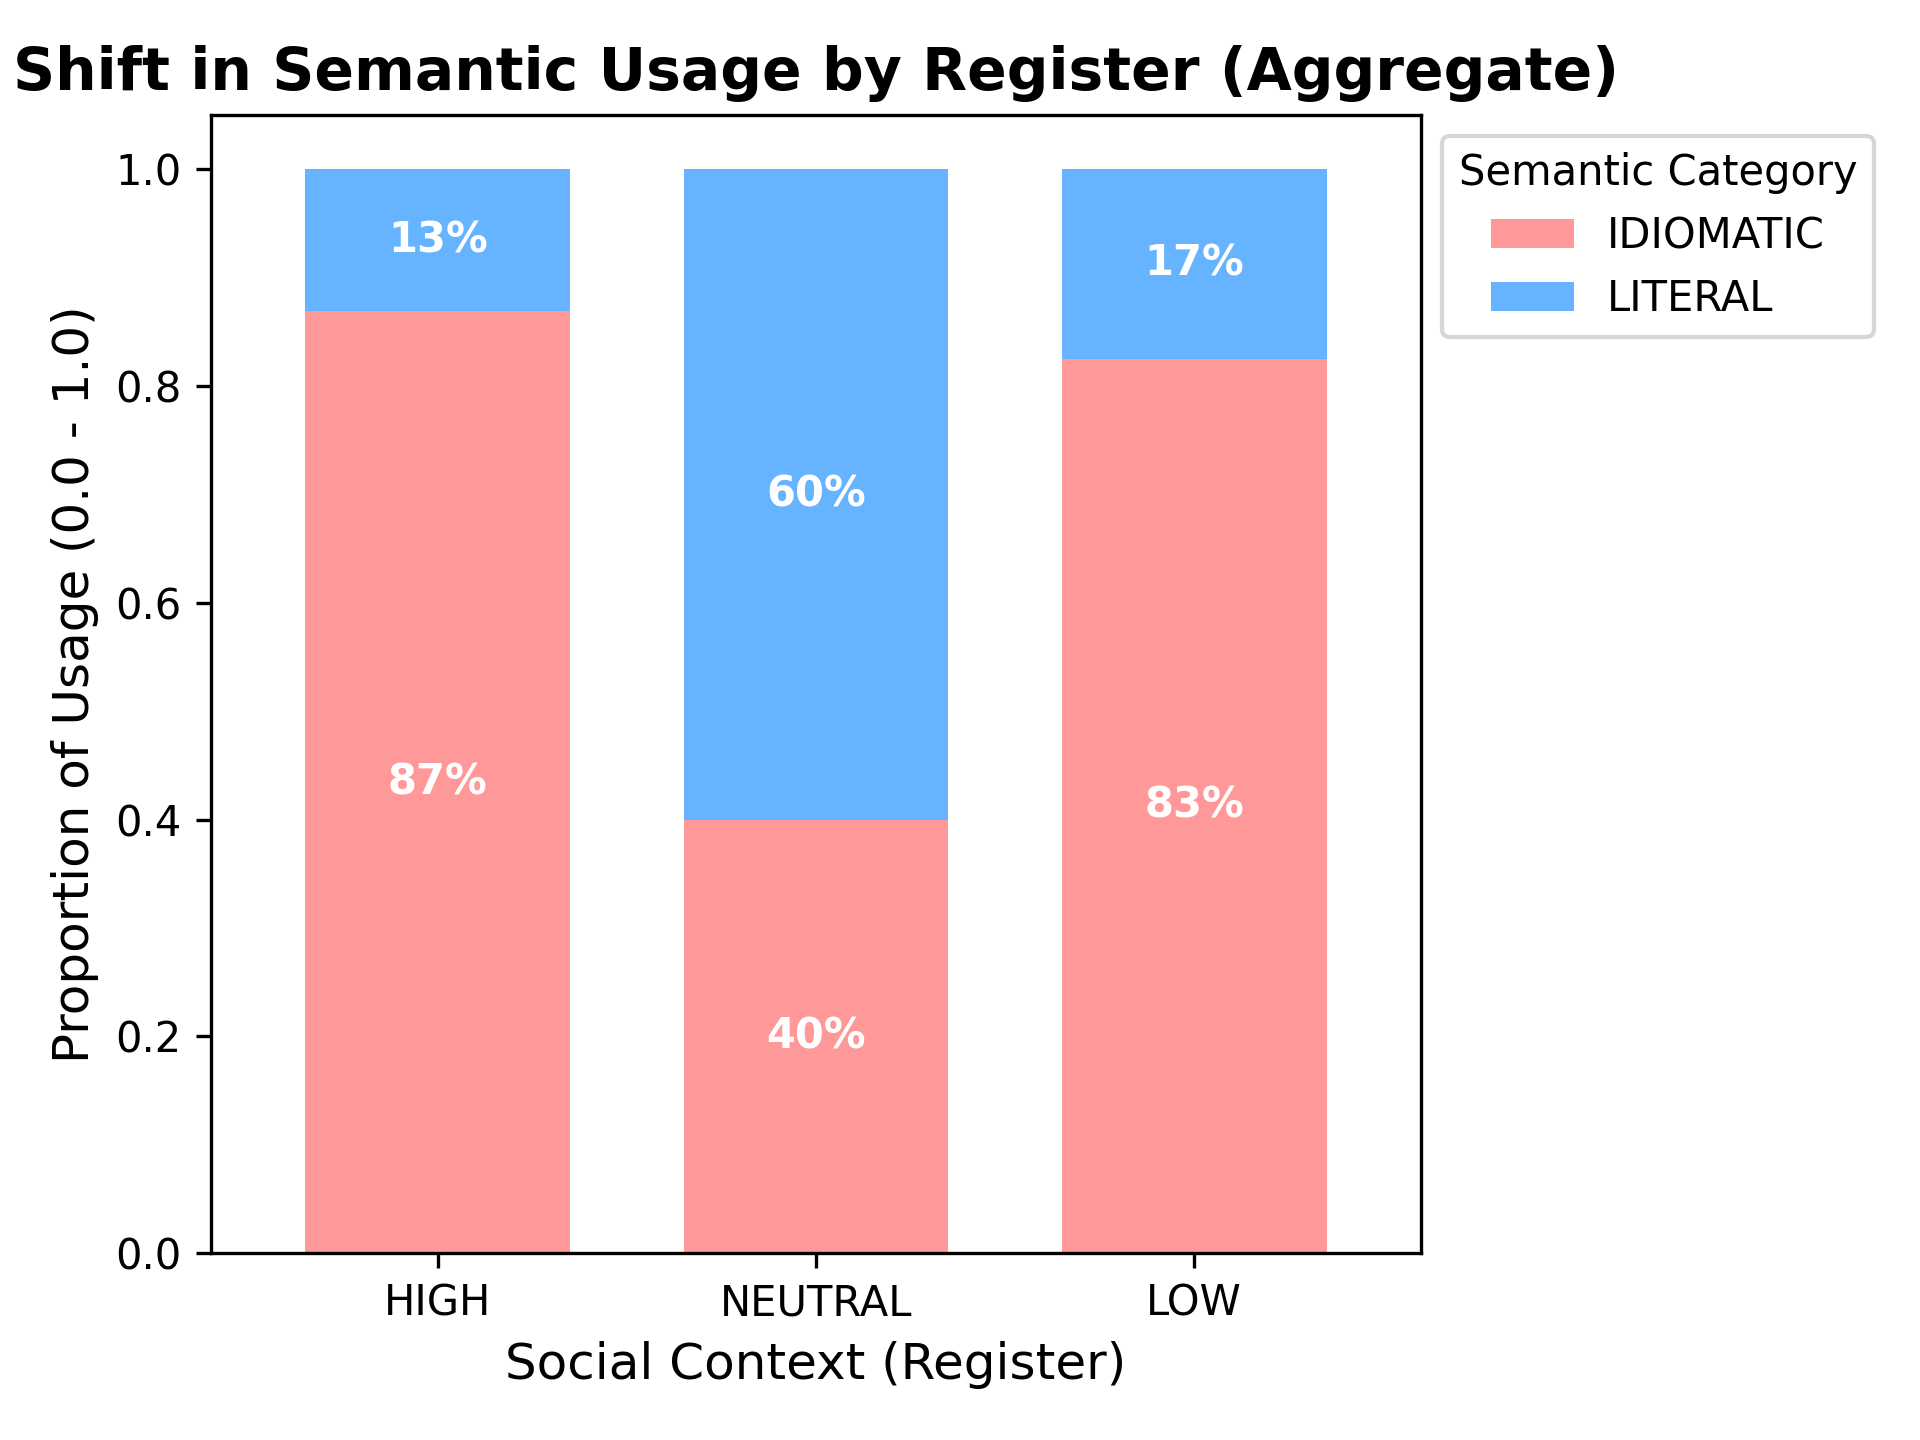
\includegraphics[width=\textwidth]{Images/results_aggregate_chart.png}
    \caption[SCC Pilot: Aggregate by Register]{Aggregate proportion of \texttt{LITERAL} vs. \texttt{IDIOMATIC} usages by register (SCC pilot data).}
    \label{fig:results-aggregate-appendix}
\end{figure}

\vspace{-0.75\baselineskip}
\begin{figure}[H]
    \centering
    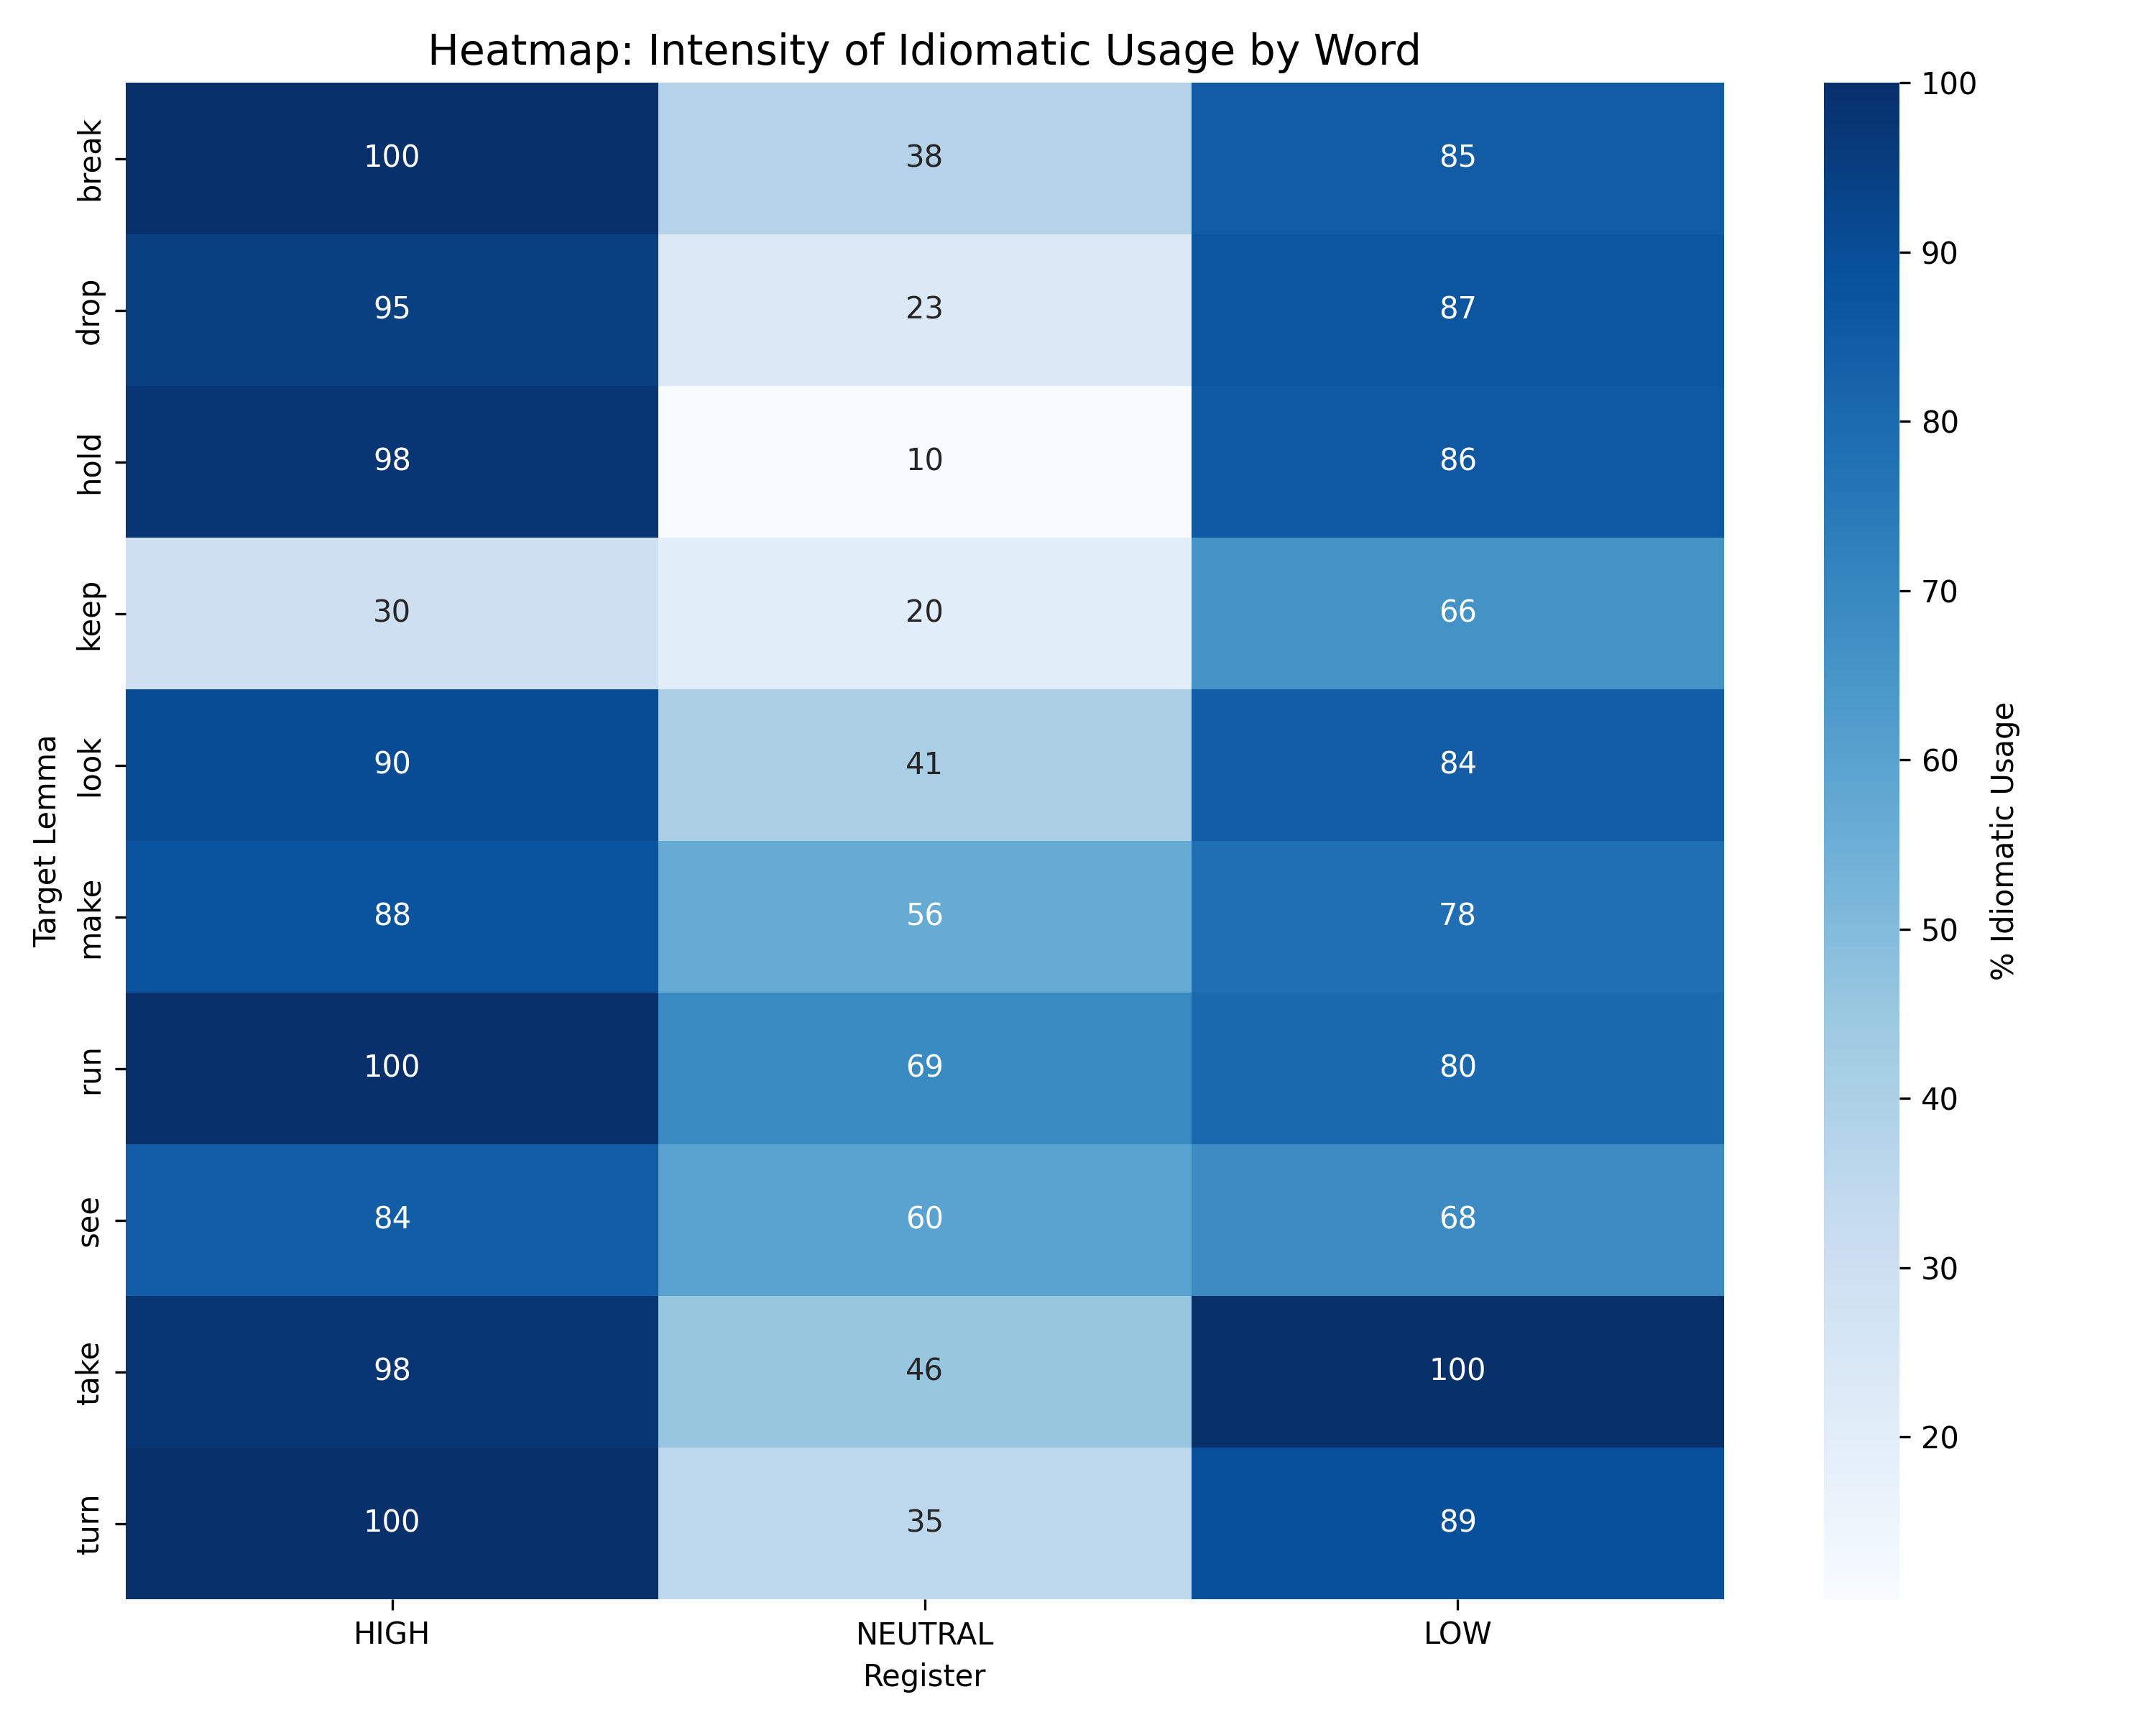
\includegraphics[width=\textwidth]{Images/results_heatmap.png}
    \caption[SCC Pilot: Idiomaticity Heatmap]{Per-lemma heatmap of \texttt{IDIOMATIC} usage rates by register (SCC pilot data).}
    \label{fig:results-heatmap-appendix}
\end{figure}

\subsection{Short Interpretation: \textit{run}}\label{subsec:interp-run}
In the pilot data, \textit{run} is classified as 100\% \texttt{IDIOMATIC} in the HIGH register. This aligns with the ``Workplace/Professional'' prompt condition: in professional contexts, \textit{run} is typically used metaphorically (e.g. \textit{run a meeting}, \textit{run tests}, \textit{run a project}) rather than to describe physical motion. For example, the synthetic HIGH-register sentence ``Could you confirm if the new software will run efficiently on older systems?'' uses \textit{run} in the sense of ``operate/function,'' i.e. a non-literal (de-lexicalised) usage.

In the LOW register, \textit{run} is 80\% \texttt{IDIOMATIC}. This is expected because casual contexts plausibly include literal movement (e.g. \textit{I ran to the store}), increasing the share of \texttt{LITERAL} uses.

\subsection{Short Interpretation: \textit{take}}\label{subsec:interp-take}
The word \textit{take} shows a V-shaped pattern. In HIGH (formal register), 98\% of uses are \texttt{IDIOMATIC}, light-verb constructions like \textit{take responsibility} or \textit{take measures}, where \textit{take} carries minimal semantic weight (e.g. from the SCC: ``Might this project take an unexpected turn given the new market analysis?''). In NEUTRAL (instructions), this drops to 46\%, with \textit{take} used literally (\textit{Take an exit}, \textit{Take one tablet}). In LOW (casual), idiomaticity rises back to 100\%, because of phrasal verbs like \textit{take off} or \textit{take it easy} (e.g. from the SCC: ``She always takes her time getting ready, it's so annoying.'').

In the SCC pilot, both formal and casual registers show high idiomaticity, while the AI-generated instructional register shows substantially lower idiomaticity. This contrast motivated the subsequent NRC comparison, whose full inferential results are reported in \nameref{sec:results}.

\clearpage
\newpage
\section{Final Dataset Visualisations}\label{sec:final-visualizations}

\vspace{1em}
\begin{figure}[htbp]
    \centering
    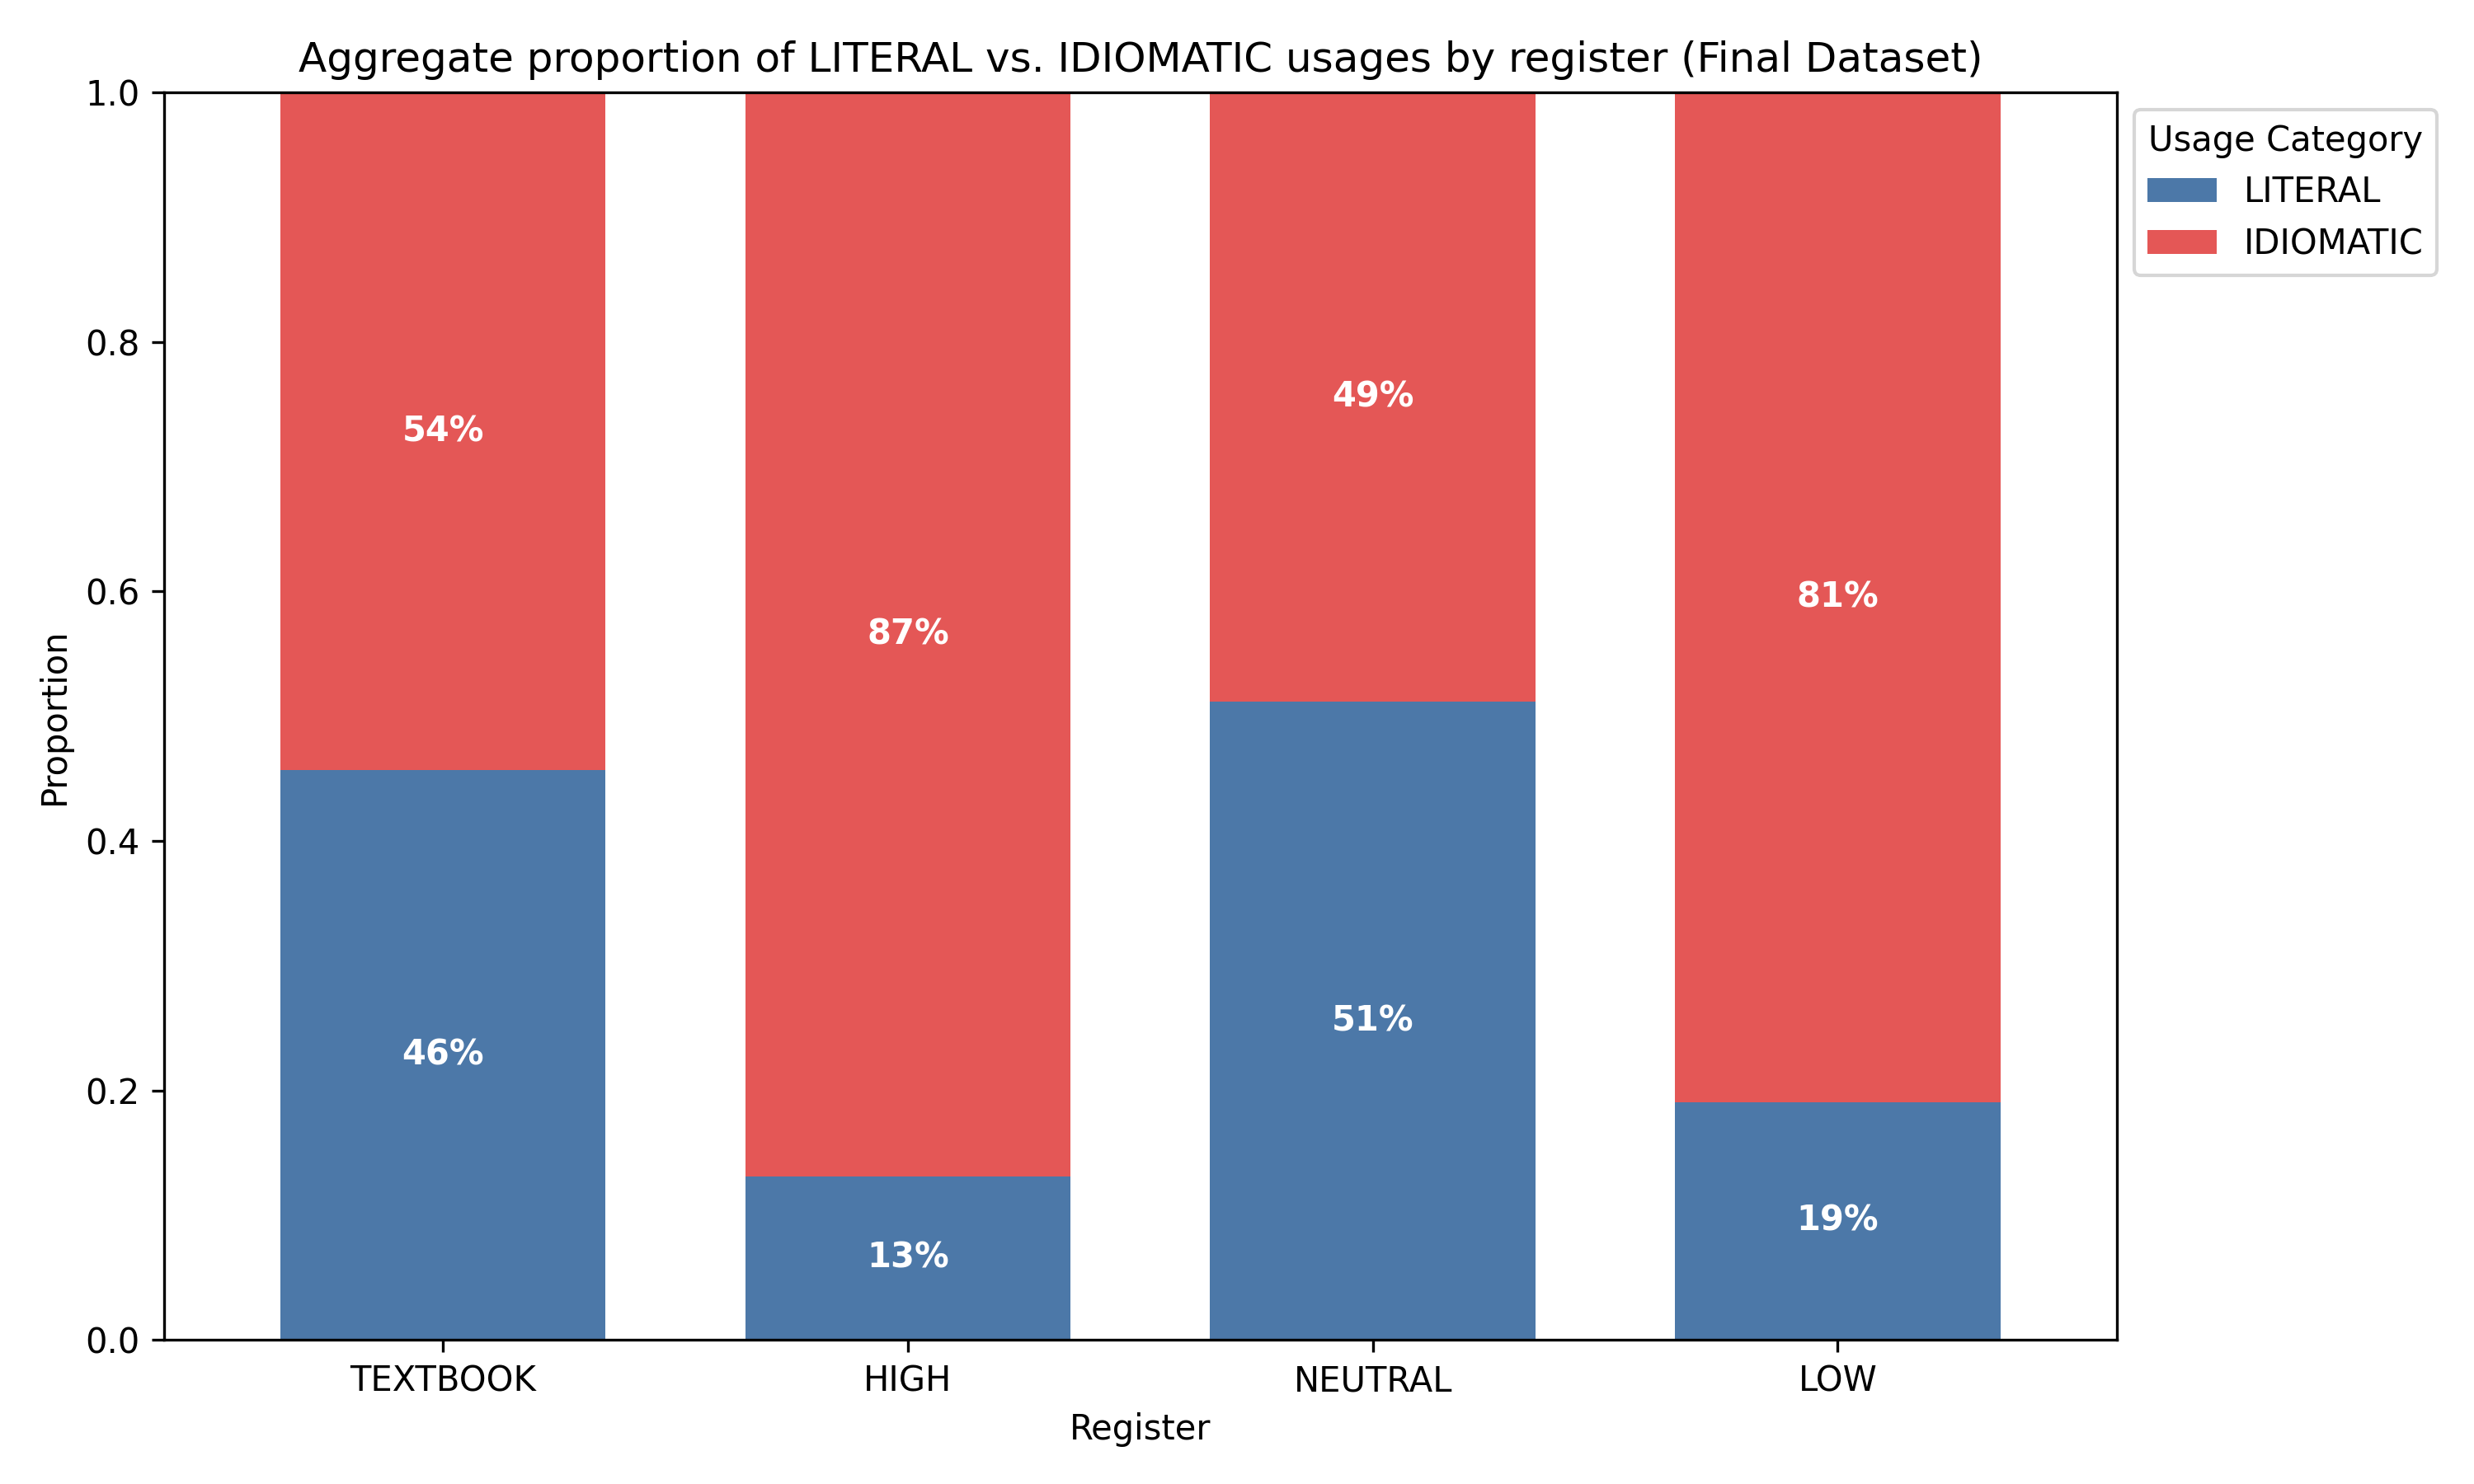
\includegraphics[width=1.0\textwidth]{Images/results_aggregate_register_proportions.png}
    \caption[Final Dataset: Aggregate by Register]{Aggregate proportion of LITERAL vs. IDIOMATIC usages by register (Final Dataset).}
    \label{fig:final_aggregate}
\end{figure}

\vspace{2em}
\begin{figure}[H]
    \centering
    % Ensure this matches your actual file name
    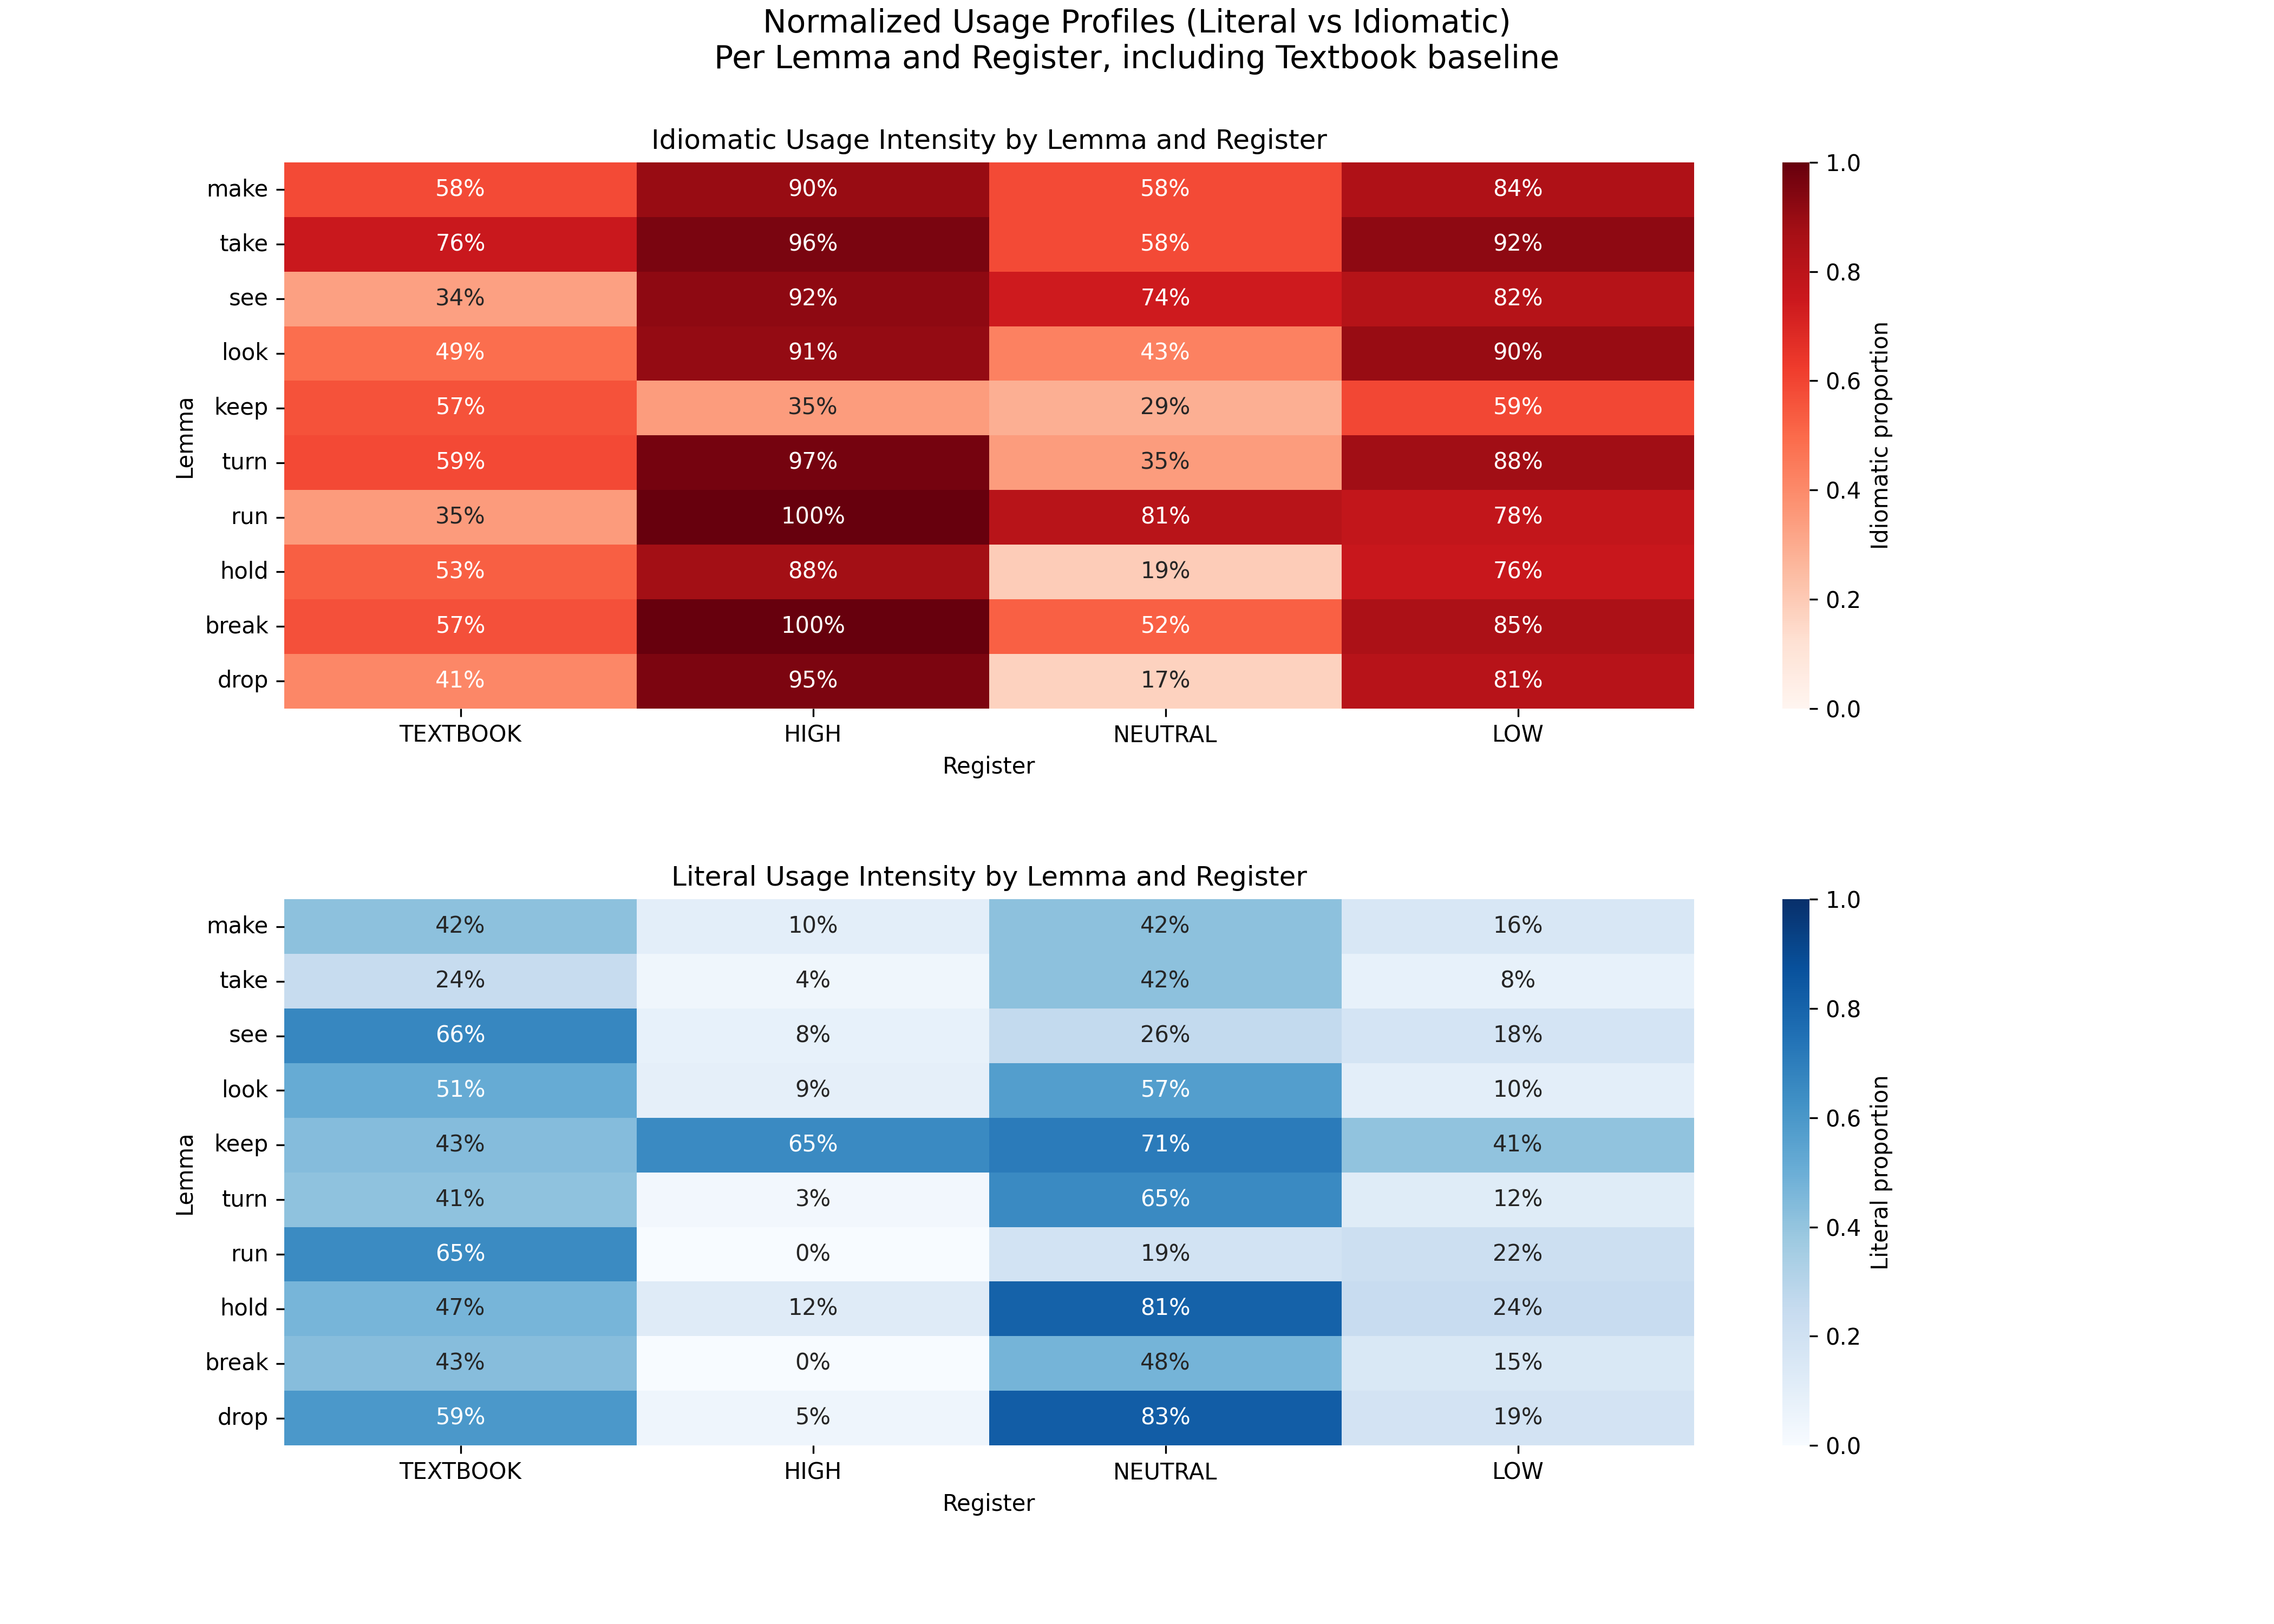
\includegraphics[width=1.0\textwidth]{Images/results_idiomaticity_heatmaps.png}
    \caption[Final Dataset: Idiomaticity Heatmap]{Per-lemma heatmap of IDIOMATIC usage rates by register (Final Dataset). Note: Cells displaying 100\% idiomaticity (e.g., \textit{run} in HIGH) are based on small cell sizes and should be interpreted with caution regarding absolute categorical boundaries.}
    \label{fig:final_heatmap}
\end{figure}

These figures provide visual representations of the final semantic classification data ($N=6,720$). Figure~\ref{fig:final_aggregate} shows the aggregate shift in idiomatic usage across prompt conditions, while Figure~\ref{fig:final_heatmap} shows the lemma-specific intensity of these phraseological shifts.

\clearpage
\section{Python Code Documentation} \label{app:python}

\subsection*{Digital Reference Appendix}

The complete computational pipeline used in this study is publicly available in the GitHub repository:

\begin{center}
\textbf{\url{https://github.com/Eidolom/llm-corpus-generation-analysis}}
\end{center}

\noindent This digital repository contains all source code, datasets, processing scripts, and version history required for full reproducibility. The project uses the following directory structure:

\vspace{0.5em}

\begin{center}
\begin{minipage}{0.8\textwidth}
\small
\begin{verbatim}
project/
|-- data/
|   |-- README.md
|   `-- target_words.txt                                # D1
|-- docs/
|   `-- DATA_ACCESS.md
|-- outputs/
|   |-- README.md
|   |-- intermediate_sentences.synthetic_backup.json
|   |-- results_aggregate_chart.png
|   |-- results_aggregate_register_proportions.csv
|   |-- results_aggregate_register_proportions.png
|   |-- results_heatmap.png
|   |-- results_idiomaticity_heatmaps.png
|   |-- results_idiomaticity_matrix.csv
|   |-- outputs/intermediate_sentences.synthetic_backup.json
|   `-- thesis_pragmatic_data_filtered_synthetic.csv
|-- src/
|   |-- README.md
|   |-- analyzers/
|   |   |-- pos_tagger.py
|   |   |-- pos_taggerNLTK_forCSV.py                    # D6
|   |   |-- pos_taggerV2NLTK.py                         # D5
|   |   |-- scalable_pos_tagger.py
|   |   |-- semantic_analyzer.py                        # D7
|   |   |-- semantic_analyzer_V2.py
|   |   |-- visualizer.py                               # D11
|   |   |-- visualizer_aggregate_register_proportions.py
|   |   `-- visualizer_idiomaticity_heatmap.py
\end{verbatim}
\end{minipage}
\vspace*{\fill}
\captionof{figure}{Directory structure (continued on page 48).}\label{fig:repo-layout-part1}
\end{center}

\begin{center}
\begin{minipage}{0.8\textwidth}
\small
\begin{verbatim}
|   |-- generators/
|   |   |-- scalable_context_generator.py               # D4
|   |   |-- scalable_context_generator_big_data.py
|   |   `-- simple_data_collector.py
|   `-- utils/
|       |-- api_config.py
|       |-- debug.py                                    # D3
|       |-- prepare_irr_annotation_sheet.py
|       |-- irr_sheet_generator.py                      # D8
|       |-- compute_split_irr.py                        # D9
|       |-- README_IRR.md
|       `-- sketch_engine_converter_nltk.py             # D2
|-- .gitattributes
|-- .gitignore
|-- LICENSE
|-- README.md
|-- SETUP.md
`-- requirements.txt
\end{verbatim}
\end{minipage}
\captionof{figure}{Directory structure (continued from page 47).}\label{fig:repo-layout-part2}
\end{center}

\subsubsection*{Code Component Index (D1--D11)}
% The D identifiers are written directly in the list for readability.
\begin{itemize}
\item \textbf{D1}: \texttt{target\_words.txt}\label{D1}
\item \textbf{D2}: \texttt{nltk\_sketch\_engine\_converter.py}\label{D2}
\item \textbf{D3}: \texttt{debug.py}\label{D3}
\item \textbf{D4}: \texttt{scalable\_context\_generator.py}\label{D4}
\item \textbf{D5}: \texttt{pos\_taggerV2NLTK.py}\label{D5}
\item \textbf{D6}: \texttt{pos\_taggerNLTK\_forCSV.py}\label{D6}
\item \textbf{D7}: \texttt{semantic\_analyzer.py}\label{D7}
\item \textbf{D8}: \texttt{src/utils/irr\_sheet\_generator.py}\label{D8}
\item \textbf{D9}: \texttt{src/utils/compute\_split\_irr.py}\label{D9}
\item \textbf{D11}: \texttt{visualizer.py}\label{D11}
\end{itemize}

\subsubsection*{Ignored Local Artifacts}

Some files are intentionally not tracked in the public repository because they are local-only configuration or derived working data.

\begin{itemize}
\item \textbf{D10}: \texttt{irr\_split\_results.csv} -- local analysis output; not committed to avoid publishing transient working results.\label{D10}
\item \texttt{irr\_annotation\_sheet.csv} and \texttt{irr\_master\_key.csv} -- IRR working files derived from copyrighted textbook material and therefore not redistributed.
\end{itemize}

\subsubsection*{Implementation Notes}

The codebase uses simplified file paths in comments for readability. The production implementation uses organised directories (\texttt{outputs/}, \texttt{data/}, \texttt{src/}) and environment variables for API keys (not hardcoded). All scripts are documented with docstrings and comments, and the repository includes a \texttt{README.md} with setup instructions, usage guidelines, and data access information. The code is modularised into analysers, generators and utilities for clarity and maintainability.

\subsubsection*{Core Logic Example: POS Filtering (pos\_taggerV2NLTK.py)}

The following snippet illustrates the core verb-filtering logic used in the pipeline:

\begin{lstlisting}[language=Python, caption={Core POS filtering logic}, label=lst:pos-core]
from nltk import word_tokenize, pos_tag
from nltk.corpus import wordnet
from nltk.stem import WordNetLemmatizer

lemmatizer = WordNetLemmatizer()
verb_tags = {'VB', 'VBD', 'VBG', 'VBN', 'VBP', 'VBZ'}

def filter_by_target_verb(sentence, target_lemma):
    tokens = word_tokenize(sentence.lower())
    pos_tags = pos_tag(tokens)
    
    for token, tag in pos_tags:
        if tag in verb_tags:
            lemma = lemmatizer.lemmatize(token, wordnet.VERB)
            if lemma == target_lemma:
                return True  # Sentence retained
    return False  # Sentence filtered out
\end{lstlisting}

\noindent For complete implementations, parameter configurations, API integration details, and full dataset processing pipelines, please refer to the GitHub repository.

\newpage
\section{Full AI Documentation}\label{sec:full-ai-docs}
\label{sec:appendix-d-prompts}

\subsection{Gemini 2.5 Flash: SCC Generation Prompts}\label{subsec:ai-scc-prompts}
\noindent{Date used:} 05/02/2026

\noindent{System Prompt}
\begin{lstlisting}
You are a linguistic expert specialising in pragmatics and corpus generation.
Your task is to generate distinct, high-quality sentences for a target word based on strict register constraints.
The sentences must be appropriate for a CEFR B1/B2 learner.
\end{lstlisting}

\noindent{Batch Prompt}
\begin{lstlisting}
Target Word: "{word}"
Batch ID: {batch_num} (Ensure these sentences are unique from generic examples)

Generate a JSON array containing exactly {3 * SENTENCES_PER_REG_PER_BATCH} sentences:

1. {SENTENCES_PER_REG_PER_BATCH} sentences: Register HIGH (Formal), Mood Question. Context: Workplace/Professional.
2. {SENTENCES_PER_REG_PER_BATCH} sentences: Register LOW (Casual), Mood Statement. Context: Friends/Personal/Slang.
3. {SENTENCES_PER_REG_PER_BATCH} sentences: Register NEUTRAL (Direct), Mood Imperative. Context: Instructions/Navigation/Rules.

Vary the sentence structure and vocabulary usage.
Output JSON keys: "register", "mood", "sentence".
\end{lstlisting}

\subsection{Gemini 2.5 Flash: Semantic Classification Prompts}\label{subsec:ai-semantic-prompts}
\noindent{Date used:} 28/02/2026

\noindent{System Prompt}
\begin{lstlisting}
You are a semantic analyzer. I will provide a list of sentences containing a target word.
Classify the usage of the target word in each sentence into exactly one category:
1. "LITERAL" (Physical/Core meaning).
2. "IDIOMATIC" (De-lexicalized, Metaphor, Phrasal Verb, or Fixed Phrase).

Return a strict JSON ARRAY of strings.
Example Output: ["LITERAL", "IDIOMATIC", "LITERAL"]
\end{lstlisting}

\noindent{Chunk Prompt}
\begin{lstlisting}
Target Word: "{word}"
Sentences to classify ({len(chunk_sentences)} items):
{json.dumps(chunk_sentences)}

Return exactly {len(chunk_sentences)} tags in a JSON array.
\end{lstlisting}

\subsection{Gemini 3 Pro: Ideation Prompt}\label{subsec:ai-ideation-prompt}
\noindent{Date used:} 20/11/2025

\begin{lstlisting}
I am starting my Bachelor's thesis in English Linguistics. I want to compare
"Textbook English" idiomaticity against sentences generated by an LLM like
Gemini. I am thinking of building two corpora and using a "High/Neutral/Low"
register distinction for the AI side to test whether it can mimic pedagogical
styles. Can you help me brainstorm a formal academic structure for this?
\end{lstlisting}

\subsection{Screenshots}\label{subsec:screenshots}
\begin{figure}[H]
    \centering
    \begin{subfigure}[t]{0.48\textwidth}
        \centering
        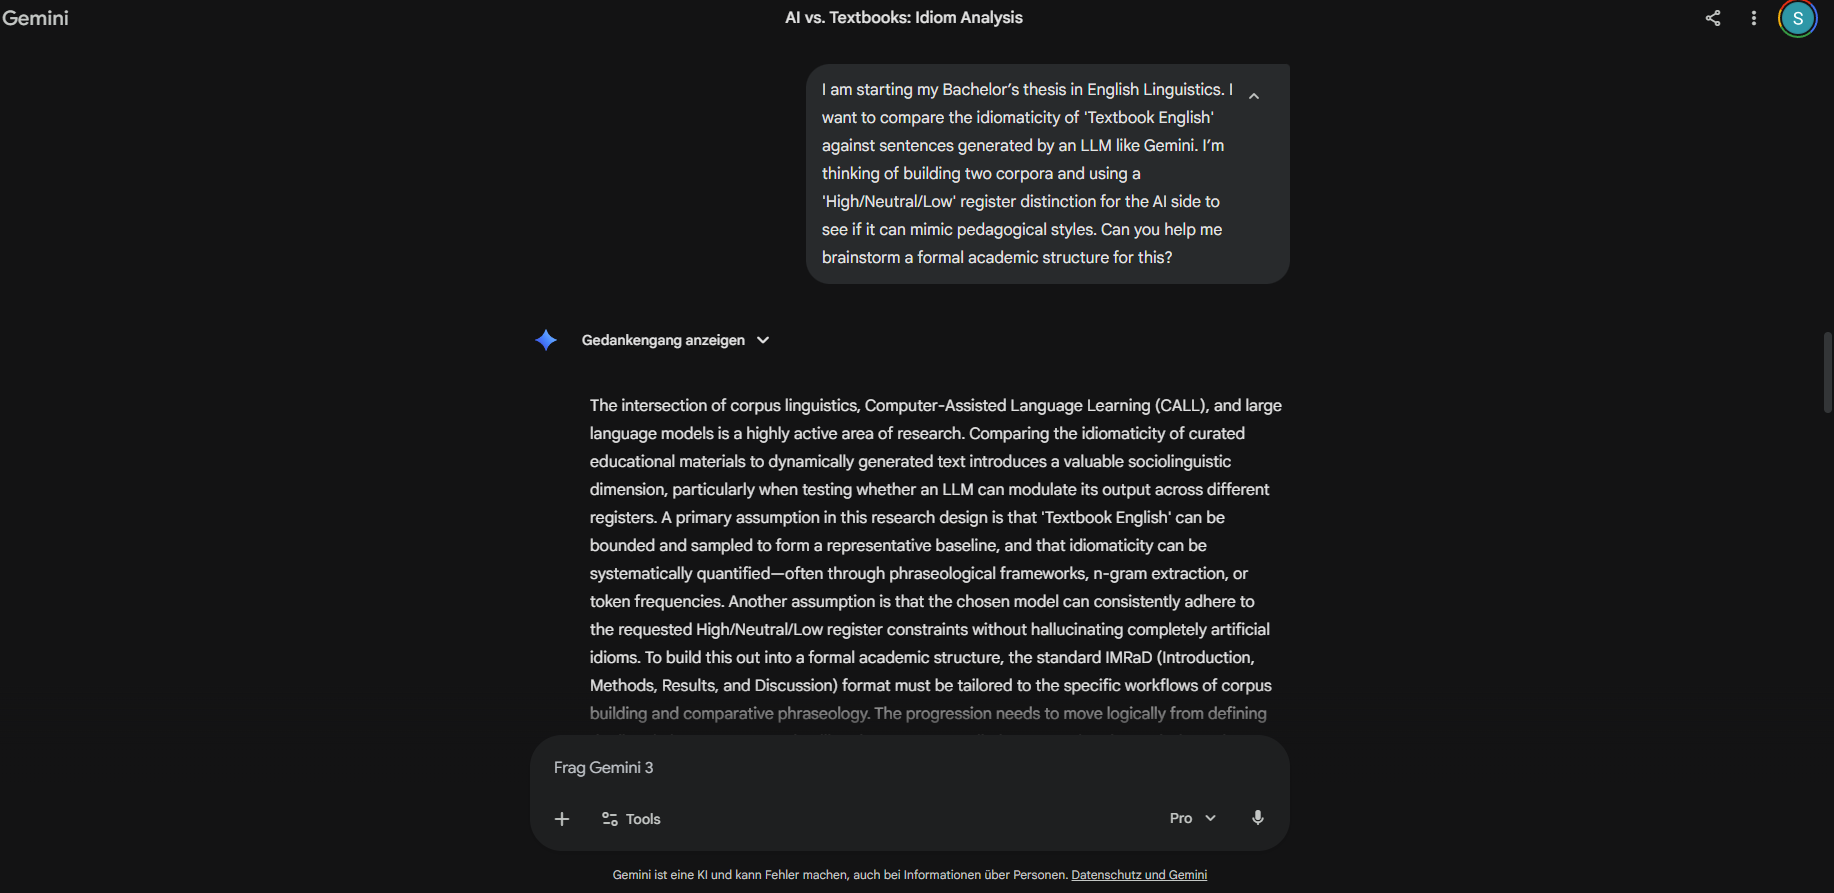
\includegraphics[width=\linewidth,clip,trim=13.0cm 0.8cm 13.0cm 0.8cm]{Screenshots/Gemini3Proof1.png}
        \caption{}
        \label{fig:gemini3-proof1}
    \end{subfigure}
    \hfill
    \begin{subfigure}[t]{0.48\textwidth}
        \centering
        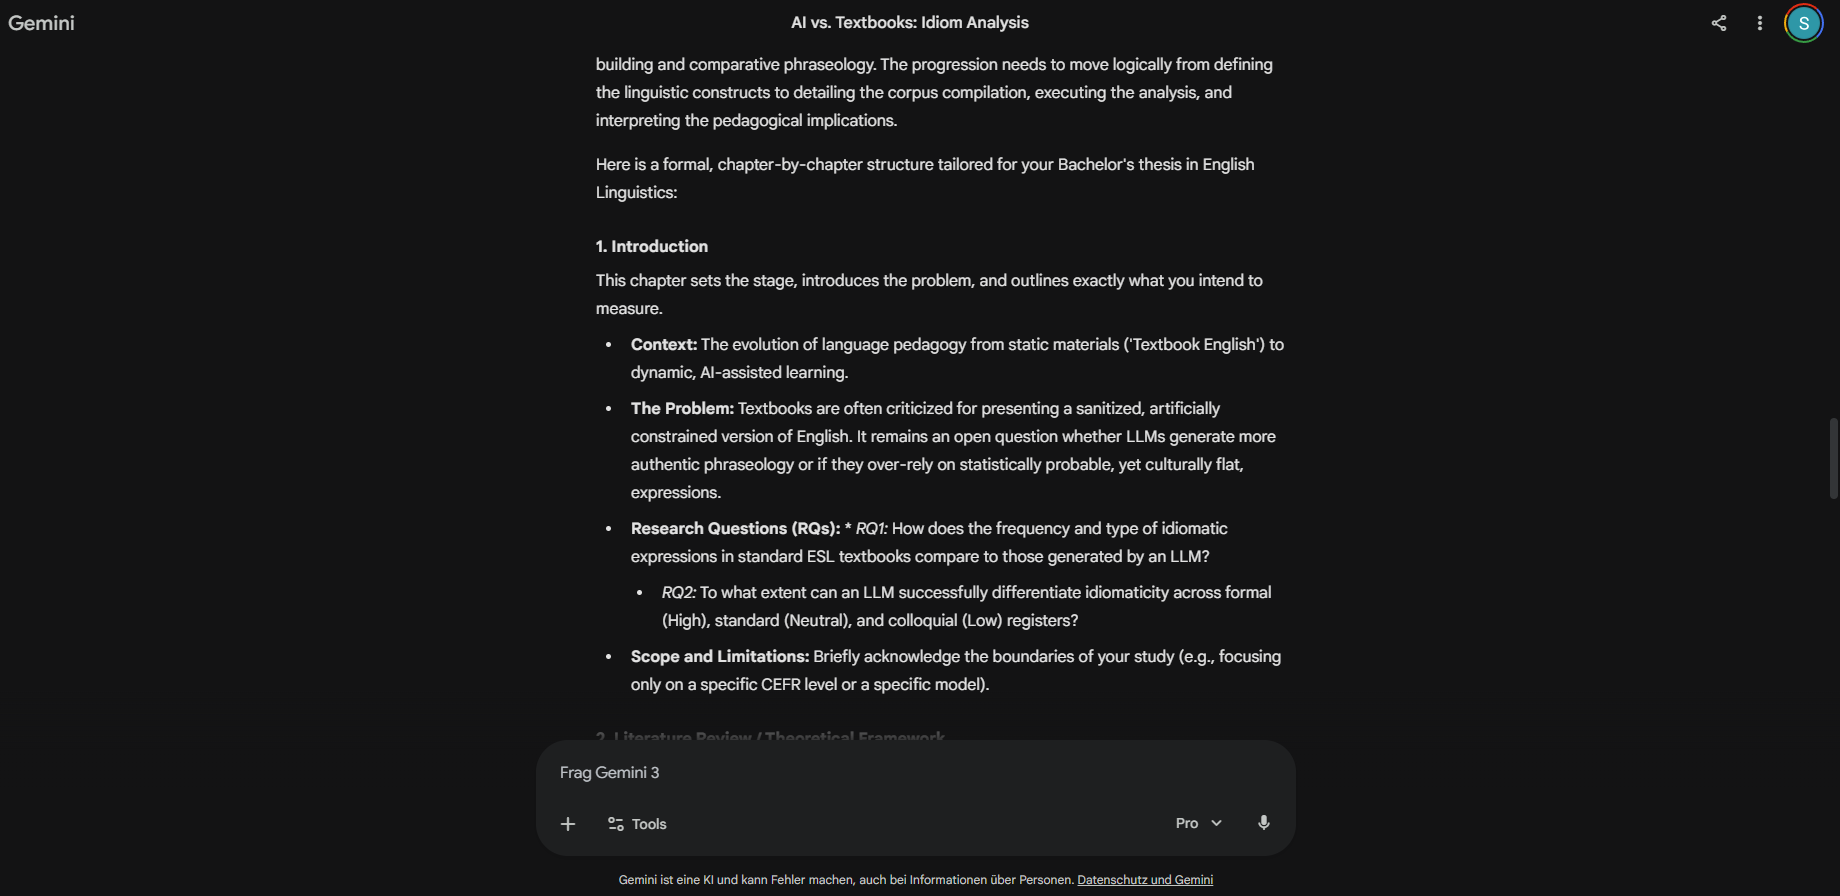
\includegraphics[width=\linewidth,clip,trim=13.0cm 0.8cm 13.0cm 0.8cm]{Screenshots/Gemini3Proof2.png}
        \caption{}
        \label{fig:gemini3-proof2}
    \end{subfigure}
    
    \vspace{0.5em}

    \begin{subfigure}[t]{0.48\textwidth}
        \centering
        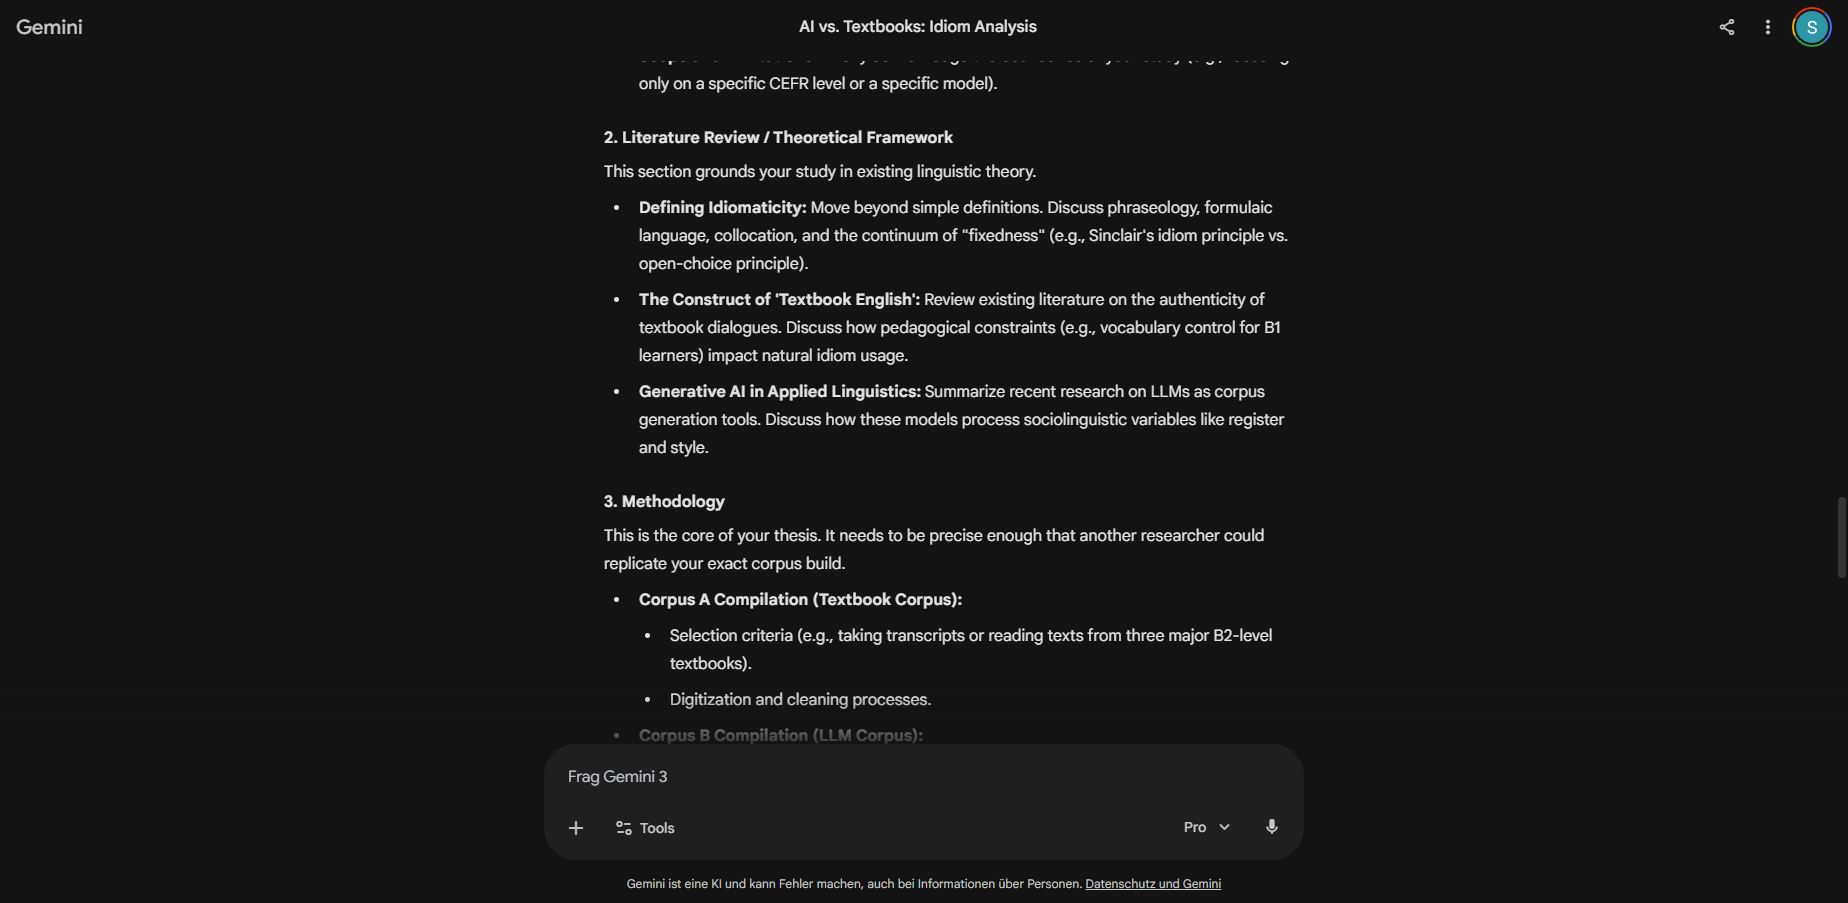
\includegraphics[width=\linewidth,clip,trim=13.0cm 0.8cm 13.0cm 0.8cm]{Screenshots/Gemini3Proof3.png}
        \caption{}
        \label{fig:gemini3-proof3}
    \end{subfigure}
    \hfill
    \begin{subfigure}[t]{0.48\textwidth}
        \centering
        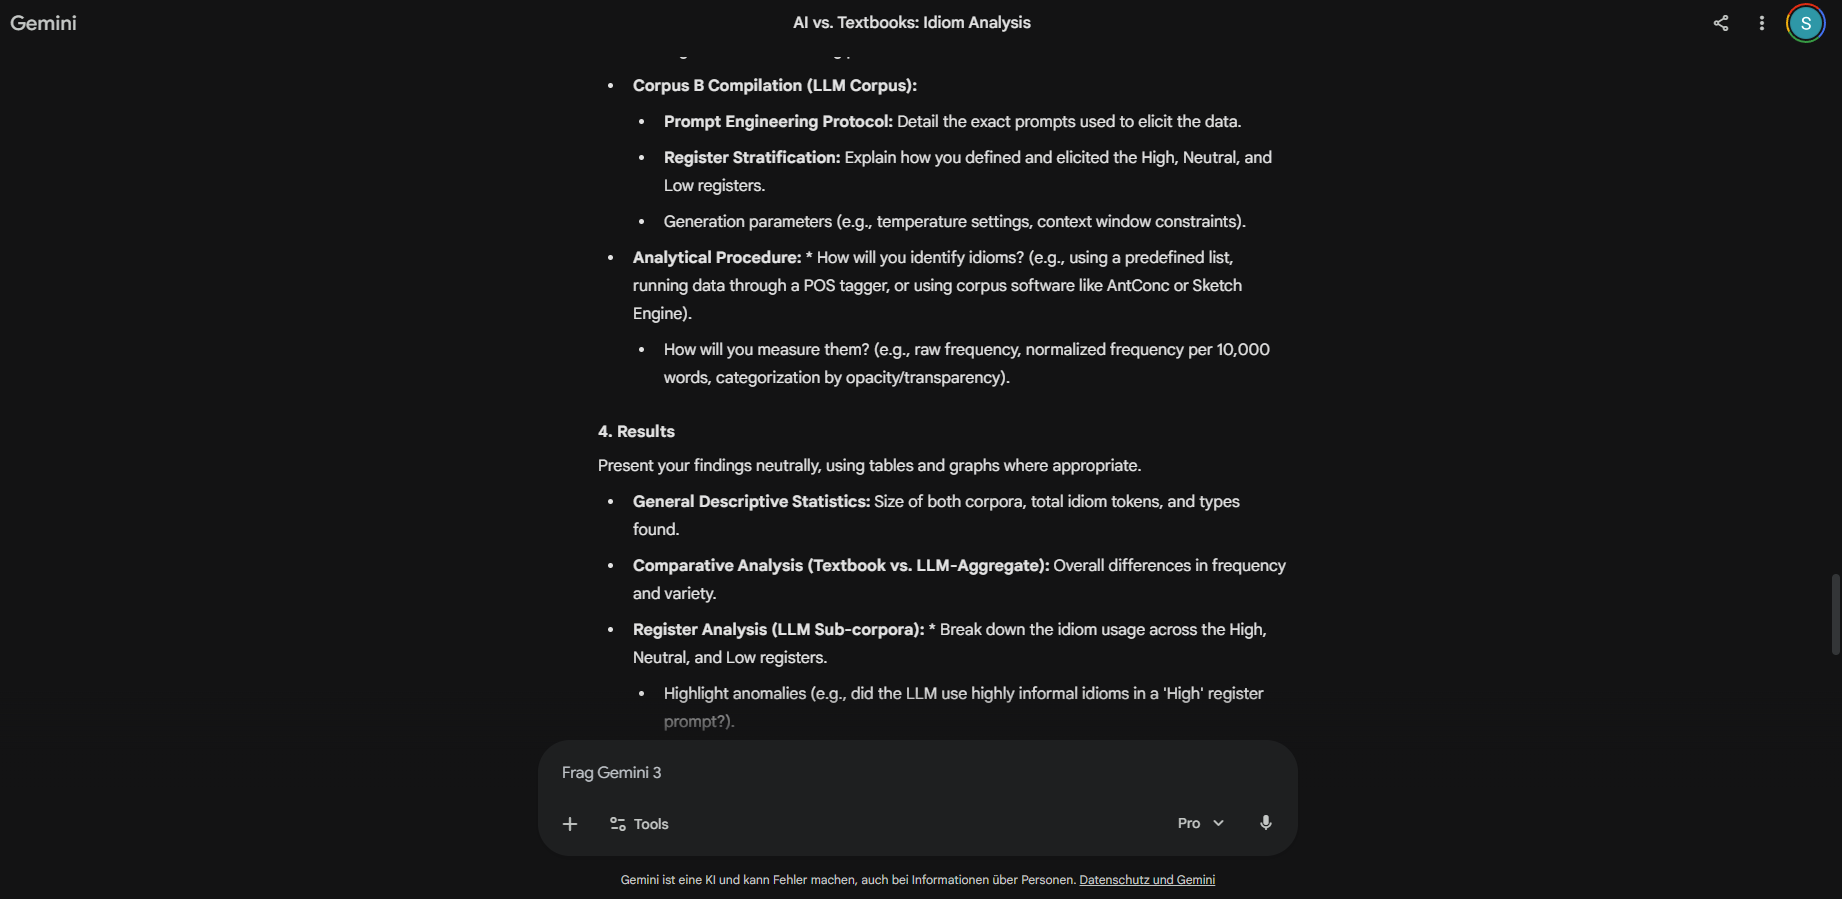
\includegraphics[width=\linewidth,clip,trim=13.0cm 0.8cm 13.0cm 0.8cm]{Screenshots/Gemini3Proof4.png}
        \caption{}
        \label{fig:gemini3-proof4}
    \end{subfigure}

    \vspace{0.5em}

    \begin{subfigure}[t]{0.48\textwidth}
        \centering
        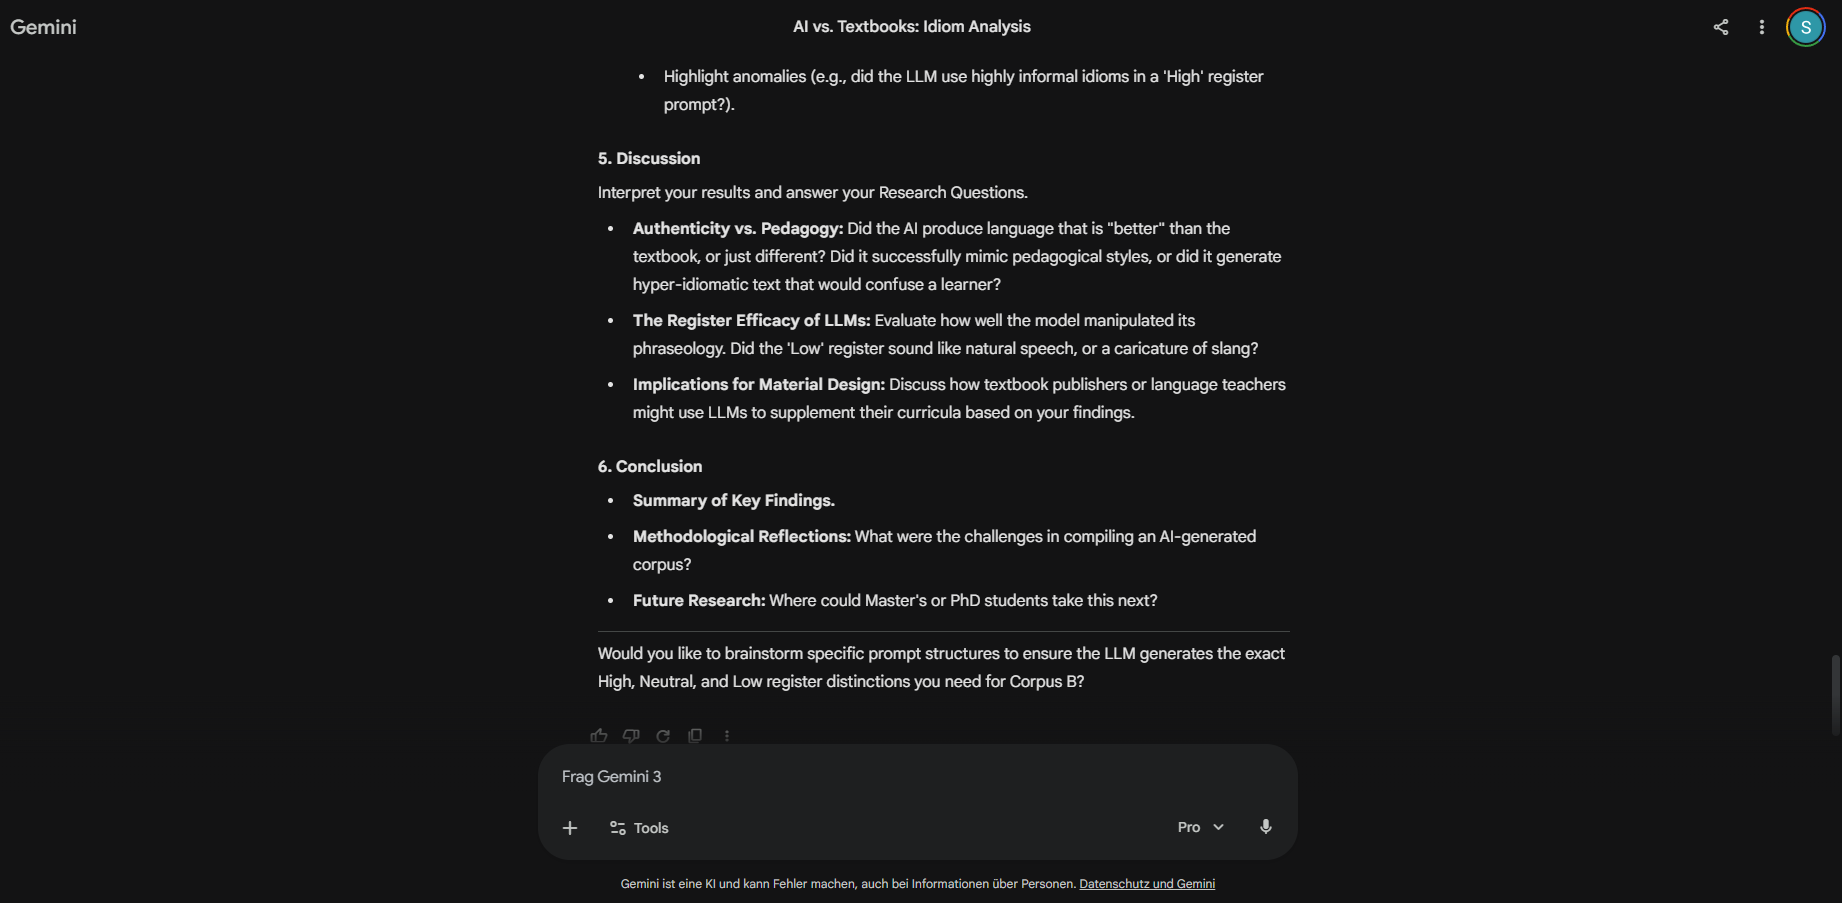
\includegraphics[width=\linewidth,clip,trim=13.0cm 0.8cm 13.0cm 0.8cm]{Screenshots/Gemini3Proof5.png}
        \caption{}
        \label{fig:gemini3-proof5}
    \end{subfigure}

    \caption[Gemini 3 Ideation Evidence Plate II]{Gemini 3 Pro screenshots documenting the broad ideation process.}
    \label{fig:gemini3-proof-plate-2}
\end{figure}

\end{document}